Um einen Überblick über das Projekt zu verschaffen und den Einstieg ins Thema der Ultraschall Phased Arrays zu erleichtern, wird zuerst das Grobkonzept vorgestellt und danach werden die damit in Verbindung stehenden Grundlagen aus der Akustik und der Signalverarbeitung erklärt.

Damit eine Objekterkennung im Raum mittels Ultraschall möglich wird, muss ein schmaler, im Winkel verstellbarer Schallkegel erzeugt werden. Dafür sind mehrere Schallquellen nötig. Wenn der Schall auf ein Objekt auftrifft, wird ein Echo erzeugt. Aus einem solchen Echo können Informationen bezüglich Distanz und Winkel des Objekts im Raum gewonnen werden. Das Grundprinzip ist in Abbildung \ref{fig:image_grundlagen_prinzip} dargestellt.

%%%%%%%%%%%%%%%%%%%%%%%%%%%%%%%%%%%%%%%%%%%%%%%%%%%%%%%%%%%%%%%%%%%%%%%%%%%%%%%%
% pictures
\begin{figure}[htb]
\begin{center}
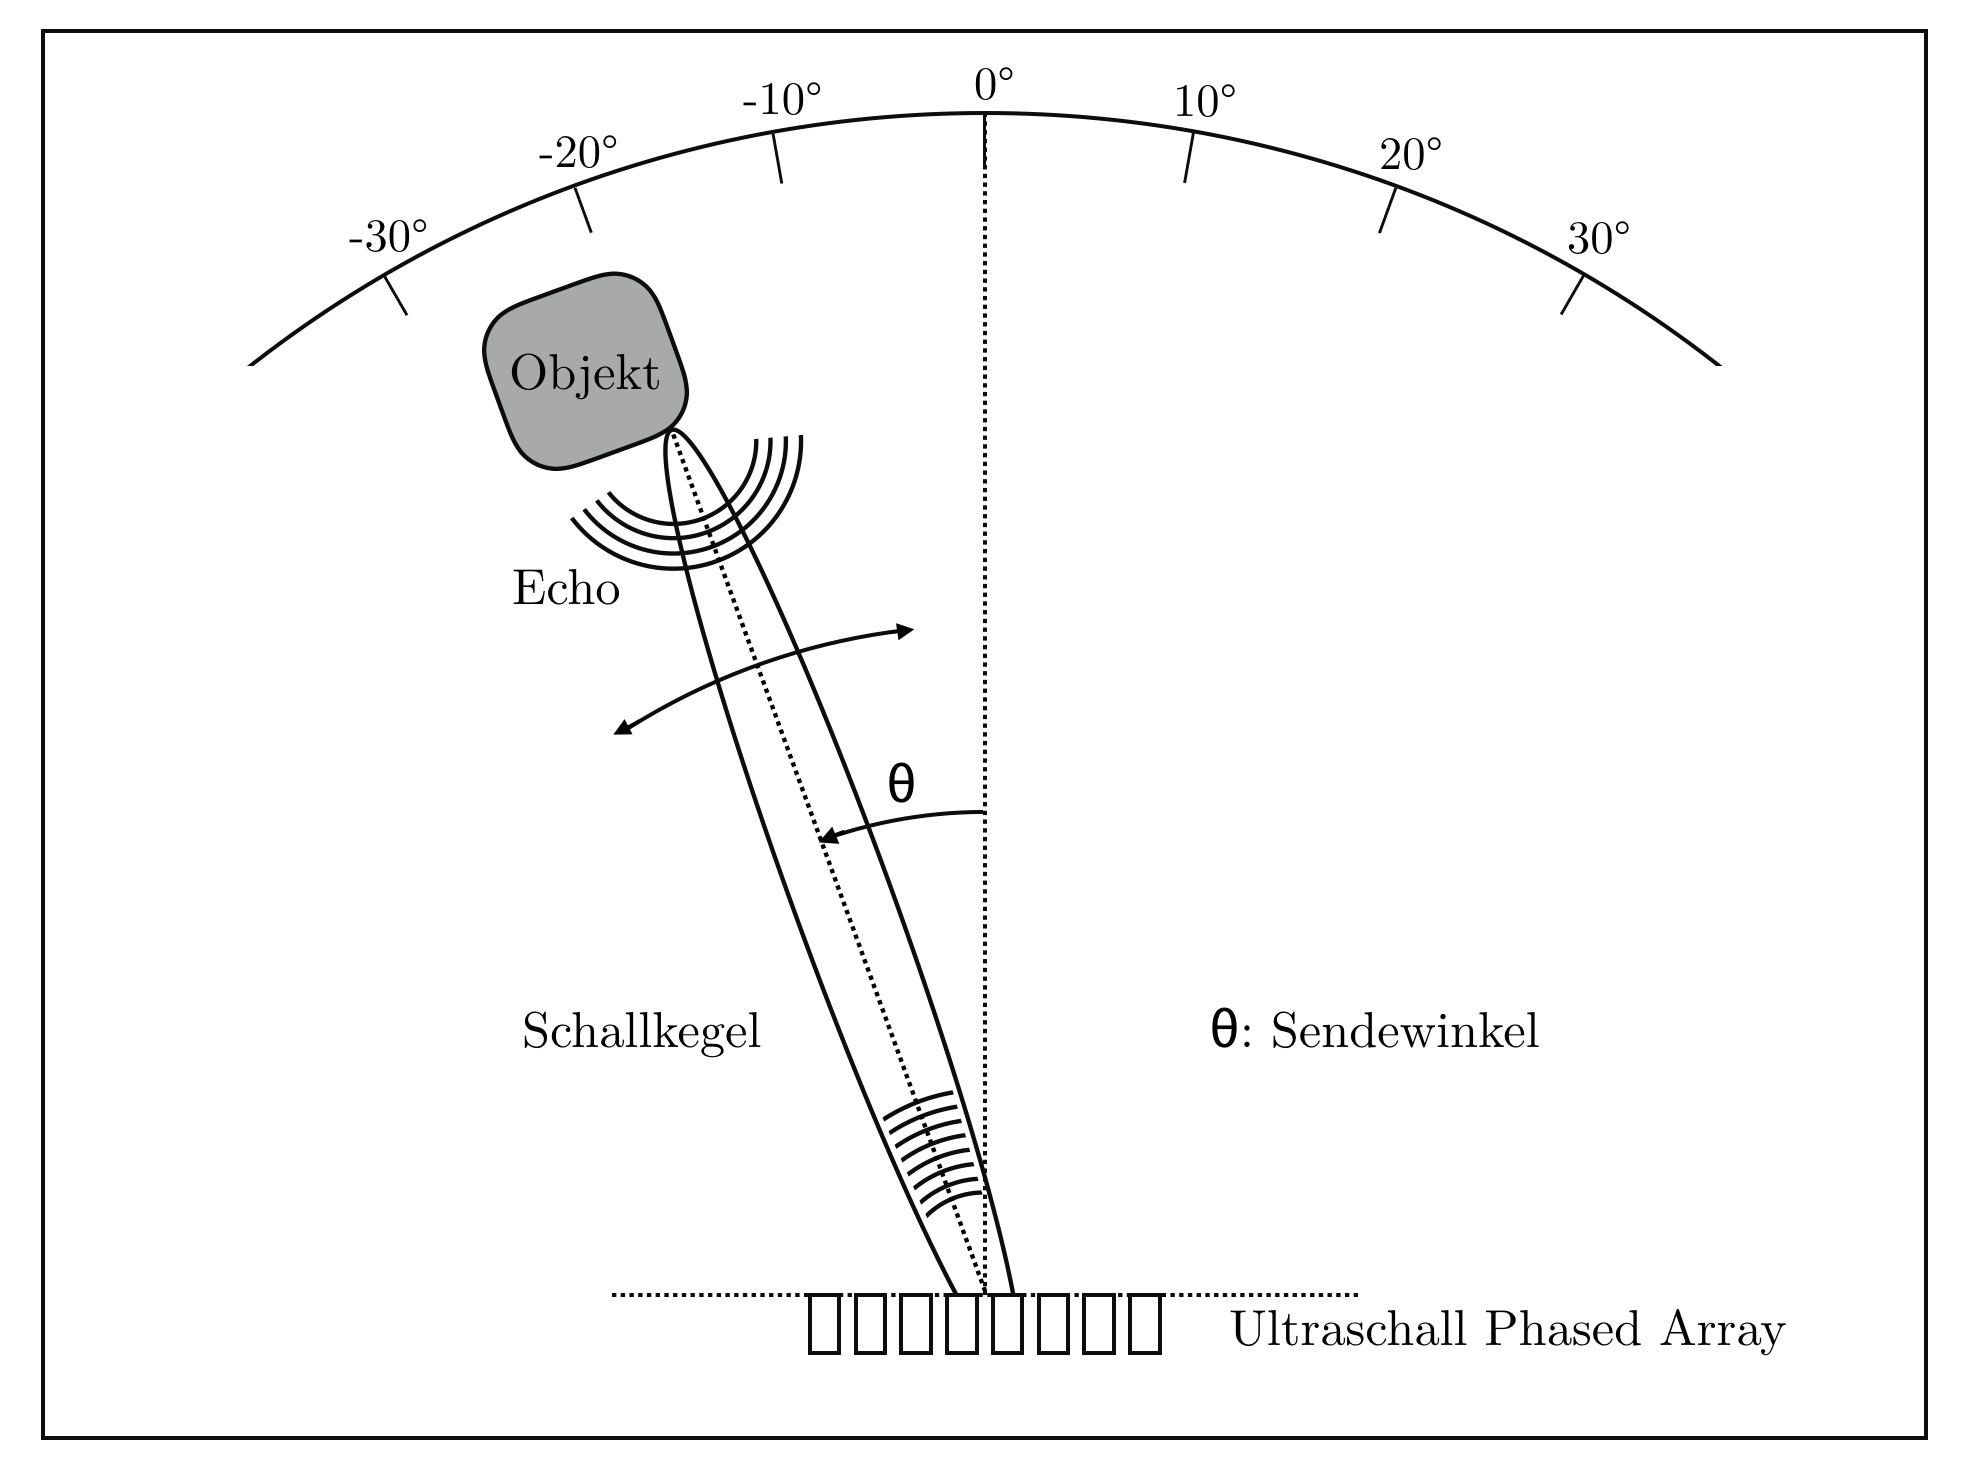
\includegraphics[width=\textwidth]{graphics/image_grundlagen_prinzip.png}
\end{center}
\caption{Prinzip eines $1$x$8$ Ultraschall Phased Array} % picture caption
\label{fig:image_grundlagen_prinzip}
\end{figure}
%
%(Abb. \ref{fig:image1})
%%%%%%%%%%%%%%%%%%%%%%%%%%%%%%%%%%%%%%%%%%%%%%%%%%%%%%%%%%%%%%%%%%%%%%%%%%%%%%%%



%%%%%%%%%%%%%%%%%%%%%%%%%%%%%%%%%%%%%%%%%%%%%%%%%%%%%%%%%%%%%%%%%%%%%%%%%%%%%%%%
%%%%%%%%%%%%%%%%%%%%%%%%%%%%%%%%%%%%%%%%%%%%%%%%%%%%%%%%%%%%%%%%%%%%%%%%%%%%%%%%
%%%%%%%%%%%%%%%%%%%%%%%%%%%%%%%%%%%%%%%%%%%%%%%%%%%%%%%%%%%%%%%%%%%%%%%%%%%%%%%%
\subsection{Grobkonzept}\label{sec:grobkonzept}
Das Ziel ist es, gerichtete Schallwellen im Raum zu erzeugen und aus deren Echos Informationen über Distanz und Winkel von Objekten im Raum zu gewinnen. Dafür wird ein System entwickelt, dass  grob in drei verschiedene Komponenten gegliedert ist:

\begin{itemize}
	\item das Ultraschall Phased Array inkl. zugehöriger Analogschaltung und deren Ansteuerung mittels Mikrocontroller
	\item ein Host-System, das die Signalverarbeitung übernimmt und als Server fungiert
	\item der Client, der als Schnittstelle zum Benutzer die Bedienung des Geräts ermöglicht und die gemessenen Resultate darstellt
\end{itemize}

In Abbildung \ref{fig:image_grundlagen_schema} wird der grobe Aufbau des Gesamtsystems dargestellt.

%%%%%%%%%%%%%%%%%%%%%%%%%%%%%%%%%%%%%%%%%%%%%%%%%%%%%%%%%%%%%%%%%%%%%%%%%%%%%%%%
% pictures
\begin{figure}[htb]
\begin{center}
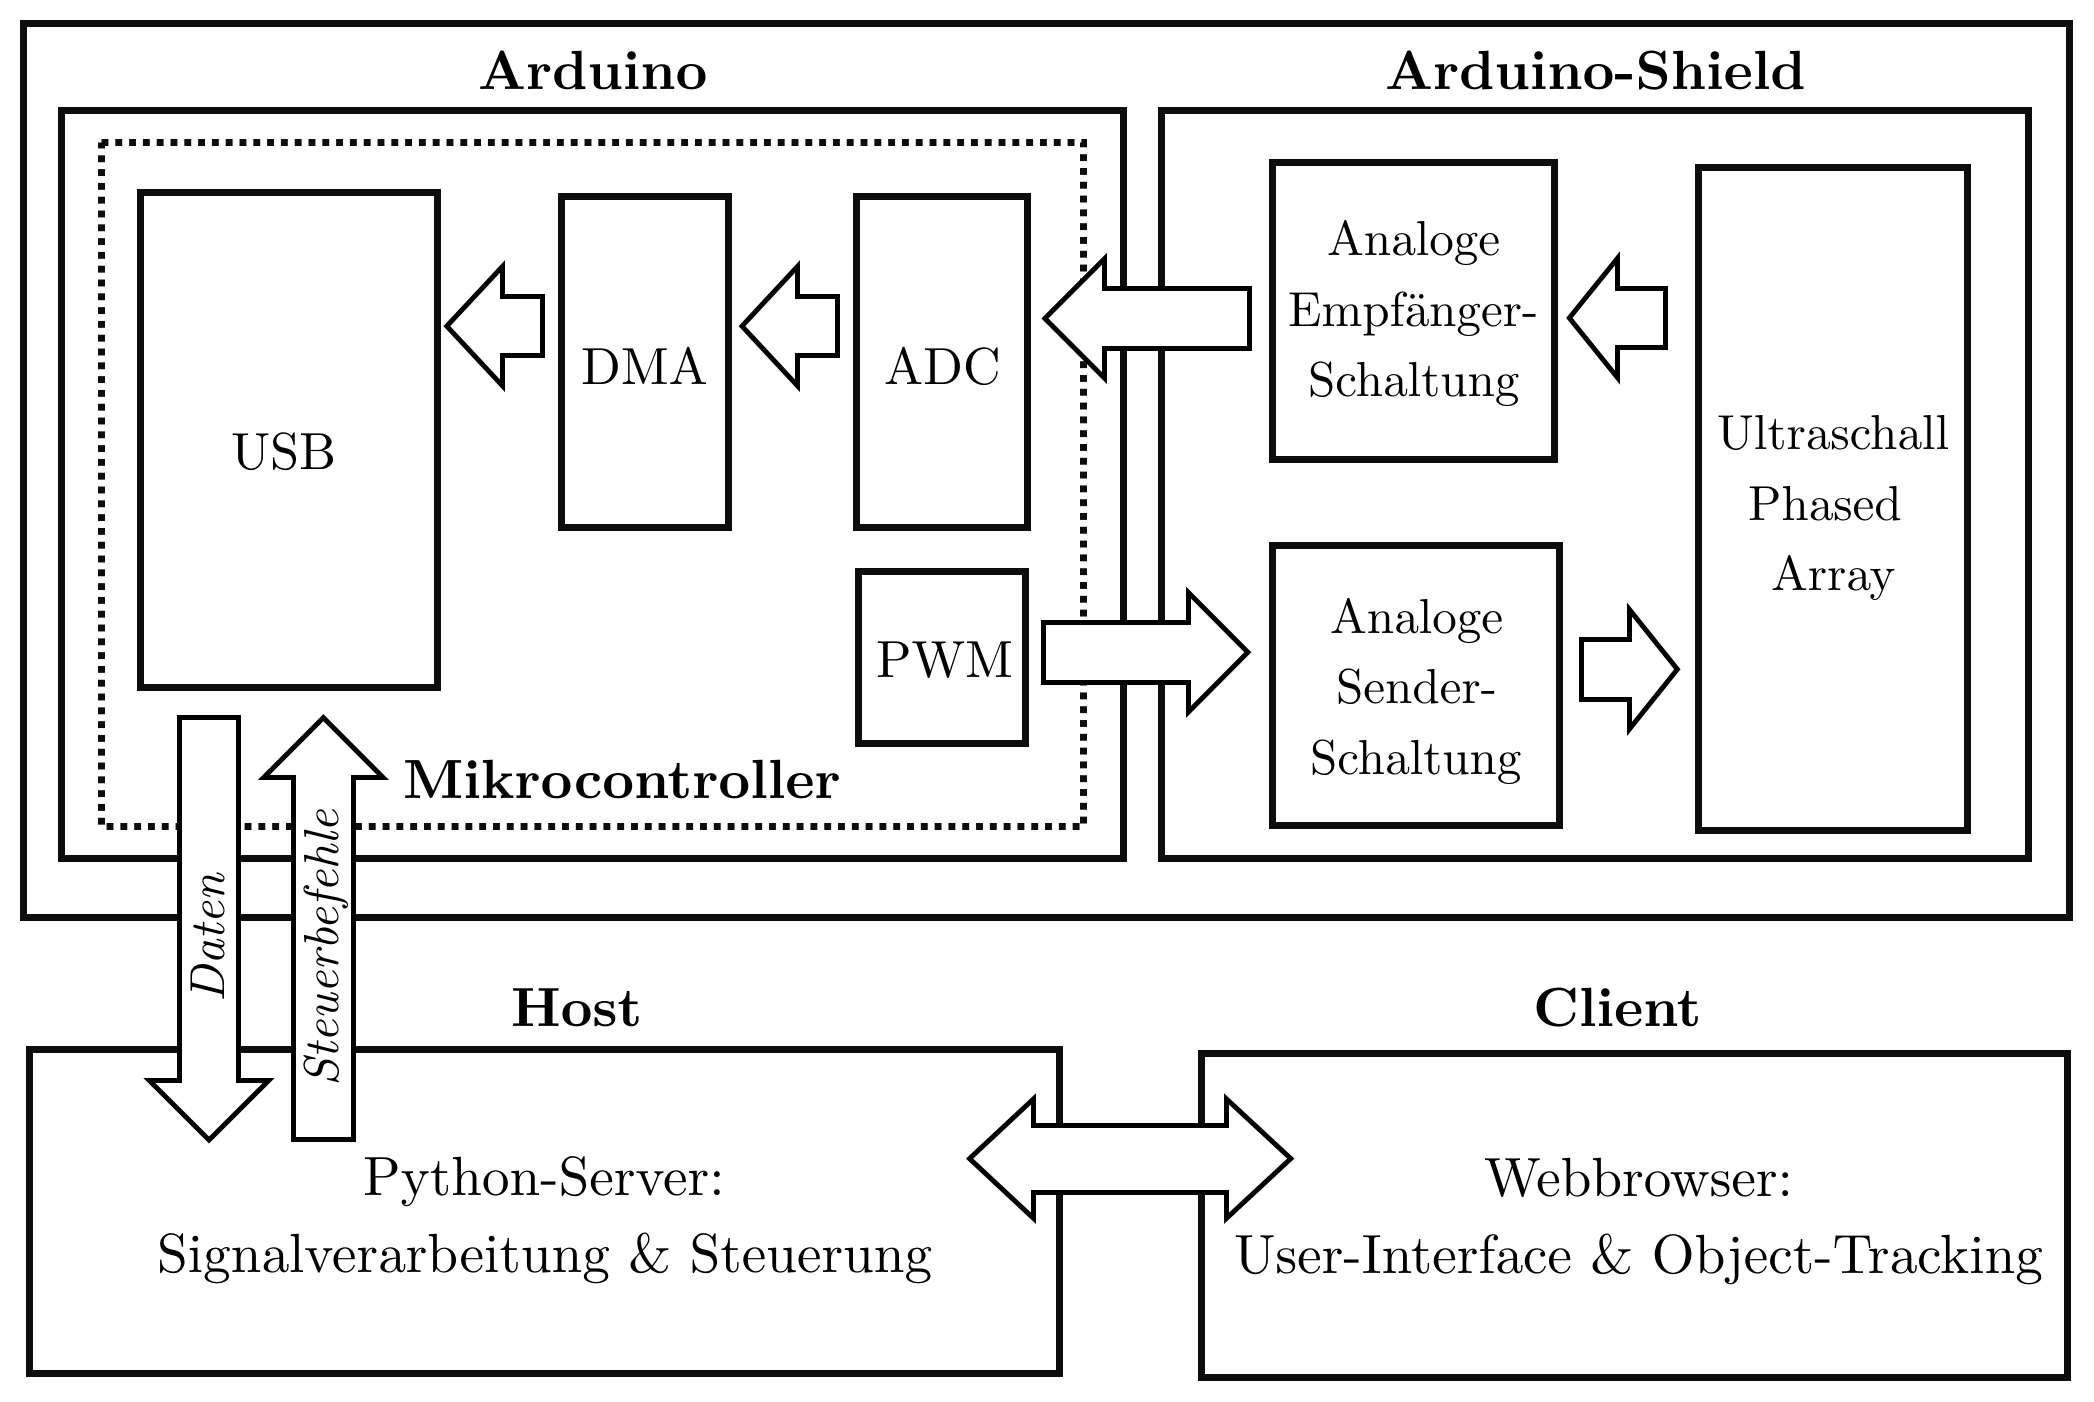
\includegraphics[width=\textwidth]{graphics/image_grundlagen_schema.png}
\end{center}
\caption{Blockschaltbild des Gesamtsystems} % picture caption
\label{fig:image_grundlagen_schema}
\end{figure}
%
%(Abb. \ref{fig:image1})
%%%%%%%%%%%%%%%%%%%%%%%%%%%%%%%%%%%%%%%%%%%%%%%%%%%%%%%%%%%%%%%%%%%%%%%%%%%%%%%%

\subsubsection{Ultraschall Phased Array und Mikrocontroller}\label{sec:utraschall_phased_array_und_mikrocontroller}
Das Phased Array wird mit Ultraschalltransceivern im Medium Luft bei einer Frequenz von $40 \mathrm{kHz}$ realisiert. Den Kern bilden die Analogschaltungen für den Empfänger und den Sender, sowie das $1$x$8$ Array aus Ultraschalltransceivern. Jeder Ultraschalltransceiver kann einzeln in Schwingung gebracht, gedämpft oder als Sensor verwendet werden. Empfangene Signale werden dabei über eine Operationsverstärkerschaltung aufbereitet. Die Funktionsweise von Ultraschall Phased Arrays und deren Eigenschaften werden in den Kapiteln \ref{sec:phased_array_schallquellen}, \ref{sec:simulationen}, \ref{sec:phased_array_sensoren} und \ref{sec:amplitudenbelegung} genauer erläutert. Die Hardware ist als Shield für das Arduino DUE Board realisiert.

Die Software für den Mikrocontroller auf dem Arduino ist nicht mithilfe der Arduino IDE entwickelt, sondern mithilfe der arm-none-eabi-toolchain. Auf dem Mikrocontroller steuert eine in der Programmiersprache C umgesetzte Statemachine die Hardware. Dabei werden über die USB-Schnittstelle Aufträge mit Details zum gewünschten Sendevorgang entgegengenommen und ausgeführt. Danach werden die digitalisierten Rohdaten der empfangenen Echos wieder per USB zurückgesendet.

Der Mikrocontroller generiert während des Sendevorgangs Signale, die danach von der Senderschaltung verstärkt und von den Schallquellen ausgesendet werden. Die Empfängerschaltung wird dabei durch rechtzeitiges Entkoppeln geschützt.

\clearpage
Ein Auftrag an den Mikrocontroller enthält folgende Informationen:

\begin{itemize}
	\item Sendewinkel
	\item Art der Amplitudenbelegung (siehe Kapitel \ref{sec:amplitudenbelegung})
	\item Anzahl Sendepulse
	\item Messzeit (Anzahl zu füllender Datenbuffer)
\end{itemize}

Die empfangenen $40 \mathrm{kHz}$-Echos werden mit einer Abtastfrequenz von $32 \mathrm{kHz}$ unterabgetastet. Dies ist möglich, weil es sehr schmalbandige Signale sind. Details zur Unterabtastung sind im Kapitel \ref{sec:abtasttheorem} genauer erläutert.\\

\subsubsection{Host}\label{sec:host}
Der Host ist als Webserver in der Programmiersprache Python realisiert. Dieser kann von einem beliebigen pythonfähigen Desktop-Betriebssystem ausgeführt werden. Entwickelt wurde die Software auf einem GNU/Linux Desktop PC, wurde aber auf verschiedenen anderen Systemen (Microsoft Windows, Raspberry Pi) erfolgreich getestet. Er ist per USB mit dem Mikrocontroller verbunden. User-Eingaben nimmt er vom Client entgegen und führt entsprechende Befehle auf der Hardware aus. Empfangene Daten werden mithilfe der digitalen Signalverarbeitung aufbereitet und zur Darstellung an den Client weitergegeben.
Damit ein gewünschter Winkelbereich automatisch gescannt werden kann, startet er auf Wunsch automatisiert die entsprechenden Aufträge über die USB-Schnittstelle und nimmt die Rohdaten entgegen. Als Webframework wird Flask verwendet.

Im Folgenden wird der Verlauf der Signalverarbeitung zusammengefasst. Die dabei verwendeten Methoden sind in den Kapiteln \ref{sec:sampling}  und \ref{sec:digitale_signalverarbeitung} detailliert beschrieben.

Die Rohdaten der $1$x$8$ Kanäle werden als erstes in den Frequenzbereich transformiert. Dabei wird das Delay korrigiert, das durch das Multiplexing während der Analog-Digital-Wandlung entsteht. Eine weitere Zeitverschiebung muss durchgeführt werden, um die gewünschte empfangsseitige Richtwirkung zu erzielen. Die Abtastrate der $1$x$8$ Kanäle wird daraufhin mittels Upsampling um den Faktor 4 erhöht. Um Rechenzeit zu sparen, wird auch das Upsampling im Frequenzbereich realisiert und die Daten danach in den Zeitbereich zurücktransformiert.
Durch die Addition der acht Signale zu einem einzigen Signal wird die oben erwähnte Richtwirkung erzielt.
Das so entstandene Signal enthält Informationen über die Position eines reflektierenden Objekts. Diese Informationen befinden sich in der Amplitude und der Zeitverschiebung von Wellenpaketen, die eine Trägerfrequenz von $40 \mathrm{kHz}$ aufweisen.
Durch die Berechnung der Enveloppe wird diese Information hervorgehoben, während das Signal ins Basisband rückt. Die Enveloppe wird durch Betragsbildung des analytischen Signals berechnet, welches mithilfe der Hilbert-Transformation erzeugt wird. Da sich das Signal im Basisband befindet, kann die Datenmenge daraufhin mit Downsampling um den Faktor 4 reduziert werden. Dieses Signal wird schlussendlich zur Darstellung an den Client gesendet.

\subsubsection{Client}\label{sec:client}
Die Bedienung des Geräts durch den Benutzer erfolgt über das User-Interface, das als Webapplikation über einen Browser aufgerufen wird. Die dabei verwendeten Programmiersprachen sind Javascript, HTML und CSS. Im User-Interface wird durch den Benutzer der zu scannende Winkelbereich ausgewählt, die Schallgeschwindigkeit festgelegt und weitere Optionen eingestellt. Sobald diese Eingaben bestätigt sind, arbeitet das mit dem Server verbundene Ultraschall Phased Array-Gerät mit den aktualisierten Einstellungen im Hintergrund. Die Signale der empfangenen Echos werden asynchron über Server-Sent-Events jeweils zum Zeitpunkt ihres Auftretens vom Client abgeholt und danach die graphischen Darstellungen aktualisiert.

Es werden zwei unterschiedliche Graphen erzeugt, welche beide zoom-/schiebbar sind und sich beim Eintreffen neuer Daten automatisch aktualisieren. Zur jeweiligen Position des Cursors werden zugehörige Daten wie Distanz oder Winkel mittels Tooltip dargestellt. Zum einen wird das aktuellste Messresultat als gewöhnlicher Linienplot dargestellt. Zum anderen wird Zeile für Zeile eine Heatmap generiert, welche die Signale farblich darstellt und so ein Bild der Umgebung erstellt, bzw. die Umgebung scannt.

Falls gewünscht, werden in Echtzeit eine variable Anzahl Maxima gesucht und auf der Heatmap mit zugehörigem Winkel und Distanz dargestellt. Dieses Maximum-Tracking ermöglicht die automatisierte Lokalisierung von Objekten im Raum.



%%%%%%%%%%%%%%%%%%%%%%%%%%%%%%%%%%%%%%%%%%%%%%%%%%%%%%%%%%%%%%%%%%%%%%%%%%%%%%%%
%%%%%%%%%%%%%%%%%%%%%%%%%%%%%%%%%%%%%%%%%%%%%%%%%%%%%%%%%%%%%%%%%%%%%%%%%%%%%%%%
%%%%%%%%%%%%%%%%%%%%%%%%%%%%%%%%%%%%%%%%%%%%%%%%%%%%%%%%%%%%%%%%%%%%%%%%%%%%%%%%
\subsection{Akustik}\label{sec:akustik}
Das Interpretieren der empfangenen akustischen Echos ist die zentrale Aufgabe bei der Datenauswertung. Es müssen gerichtete Ultraschallwellen ausgesendet werden und anhand der empfangenen Echos Informationen über Distanz und Winkel gewonnen werden. Dabei bezeichnet Ultraschall nicht mehr hörbaren Schall, welcher einen Frequenzbereich von etwa $20 \mathrm{kHz}$ bis $10 \mathrm{GHz}$ umfasst. Schall mit höherer Frequenz wird als Hyperschall bezeichnet \cite{KOHLRAUSCH}.

\subsubsection{Wellengleichung für akustische Schwingungen}\label{sec:wellengleichung_fuer_akustische_schwingungen}
Ultraschall Phased Arrays machen sich die Wellencharakteristik von Schall zunutze. Im Folgenden wird deshalb die Herleitung der Ausbreitung von Schall im Raum erklärt. Schallwellen sind mechanische Schwingungen, die sich in Festkörpern, Gasen oder Flüssigkeiten ausbreiten. In Festkörpern können sich Schallwellen sowohl longitudinal als auch transversal zur Ausbreitungsrichtung bewegen im Gegensatz zu Fluiden, wo nur longitudinale Wellen vorkommen.
Sie lassen sich mit verschiedenen Grössen beschreiben, welche die Ausbreitung der Welle in Abhängigkeit der Zeit und des Orts definieren. Dafür werden oft die Druckschwankung $p(r,t)$ um den Umgebungsdruck $p_{0}$ , die Dichteschwankung $\rho(r,t)$ um die Umgebungsdichte $\rho$ oder die Schallschnelle $v(r,t)$ verwendet.

Die Herleitung der Wellengleichung, welche die Ausbreitung von Schall in einem Medium beschreibt, setzt kleine Schwankungen der oben erwähnten Grössen im Vergleich mit $p_{0}$, $\rho$ und der Schallgeschwindigkeit voraus. Sie wird aus drei Grundgleichungen zusammengesetzt. Die folgende Herleitung beschränkt sich auf die Beschreibung des Schalls in $x$-Richtung im dreidimensionalen Raum.

Die Bewegungsgleichung \eqref{eq:bewegungsgleichung} ergibt sich aus der Eulerschen Gleichung für die Rotation eines starren Körpers. Sie beschreibt die Beschleunigung eines kleinen Volumenelementes mit Dicke $dx$ und den Seitenflächen $dy \cdot dz$. Eine senkrechte Druckausübung mit $p(x)$ auf der einen Seitenfläche und $-p(x+dx)$ auf der anderen kann weder ein Drehmoment noch eine Rotationsbeschleunigung auslösen. Deshalb wird das Volumenelement auf beiden Seitenflächen gleich beschleunigt \cite{LOOSER}:

%%%%%%%%%%%%%%%%%%%%%%%%%%%%%%%%%%%%%%%%%%%%%%%%%%%%%%%%%%%%%%%%%%%%%%%%%%%%%%%%
\begin{equation}
\begin{gathered}
\rho \cdot dy\cdot dz \cdot dx \cdot \frac{\partial v}{\partial t} = (p(x)-p(x+dx))\cdot dy\cdot dz\\ \rho \cdot \frac{\partial v}{\partial t} = - \frac{\partial p}{\partial x}
\end{gathered}\label{eq:bewegungsgleichung}
\end{equation}
%%%%%%%%%%%%%%%%%%%%%%%%%%%%%%%%%%%%%%%%%%%%%%%%%%%%%%%%%%%%%%%%%%%%%%%%%%%%%%%%

Die Änderung des Drucks auf das Volumenelement $V=\Delta x \cdot dy\cdot dz$ verursacht eine zeit\-liche Volumenänderung. Der Geschwindigkeitsgradient $dv/dx$ beschreibt die örtliche Änderung der Verformungsgeschwindigkeit eines Körpers (in diesem Fall das Volumenelement $V$) in $x$-Richtung. Über die Kontinuitätsgleichung lässt sich dieser Geschwindigkeitsgradient mit der zeitlichen Volumenänderung verknüpfen. Dabei beschreiben $v_{1}$ und $v_{2}$ die Geschwindigkeiten der beiden Seitenflächen  des Volumenelements $V$ und $S = dy \cdot dz$ deren Fläche. Gemäss \cite{HERING} folgt:

%%%%%%%%%%%%%%%%%%%%%%%%%%%%%%%%%%%%%%%%%%%%%%%%%%%%%%%%%%%%%%%%%%%%%%%%%%%%%%%%
\begin{equation}
\begin{gathered}
\frac{\partial V}{\partial t} = \frac{V(t_{1}+\partial t)-V(t_{1})}{\partial t}= \frac{ S \cdot (\Delta x + (v_{2}-v_{1})\cdot \partial t) - S \cdot \Delta x} {\partial t} \\
= \frac{ S \cdot \Delta x + S \cdot ((v_{1}+ \frac{\partial v}{\partial x}\cdot \Delta x)-v_{1}) \cdot \partial t - S \cdot\Delta x} {\partial t} \\
\frac{\partial V}{\partial t} = V \cdot \frac{\partial v}{\partial x}
\end{gathered}\label{eq:kontinuitätsgleichung}
\end{equation}
%%%%%%%%%%%%%%%%%%%%%%%%%%%%%%%%%%%%%%%%%%%%%%%%%%%%%%%%%%%%%%%%%%%%%%%%%%%%%%%%

Das Kompressionsmodul $K$ ist eine Materialeigenschaft und beschreibt die Volumenänderung $dV$ bei einer Druckänderung $dp$. Es wird beschrieben durch:
%%%%%%%%%%%%%%%%%%%%%%%%%%%%%%%%%%%%%%%%%%%%%%%%%%%%%%%%%%%%%%%%%%%%%%%%%%%%%%%%
\begin{equation}
\begin{gathered}
\frac{\partial V}{\partial p} = -\frac{V}{K}\\
\frac{\partial V}{\partial t} = -\frac{V}{K} \cdot \frac{\partial p}{\partial t}
\end{gathered}\label{eq:kompressionsmodul}
\end{equation}
%%%%%%%%%%%%%%%%%%%%%%%%%%%%%%%%%%%%%%%%%%%%%%%%%%%%%%%%%%%%%%%%%%%%%%%%%%%%%%%%

Werden (\ref{eq:kontinuitätsgleichung}) und (\ref{eq:kompressionsmodul}) gleichgesetzt, so entsteht ein Zusammenhang zwischen dem Geschwindigkeitsgradienten und der zeitlichen Druckveränderung. Wird dieser Zusammenhang nach der Zeit und die Bewegungsgleichung nach $x$ abgeleitet, so können diese drei Grundgleichungen zur Wellengleichung \ref{eq:wellengleichung} zusammengefasst werden \cite{HERING}.

%%%%%%%%%%%%%%%%%%%%%%%%%%%%%%%%%%%%%%%%%%%%%%%%%%%%%%%%%%%%%%%%%%%%%%%%%%%%%%%%
\begin{equation}
\begin{gathered}
\frac{\partial ^{^{2}}p}{\partial t^{2}}=\frac{K}{\rho} \cdot \frac{\partial ^{^{2}}p}{\partial x^{2}}
\end{gathered}\label{eq:wellengleichung}
\end{equation}
%%%%%%%%%%%%%%%%%%%%%%%%%%%%%%%%%%%%%%%%%%%%%%%%%%%%%%%%%%%%%%%%%%%%%%%%%%%%%%%%

In dieser Differentialgleichung 2. Ordnung ist nur der Druck abhängig von Ort und Zeit. Sie beschreibt die Ausbreitung von akustischen Wellen. Lösungen dieser Wellengleichung sind alle Funktionen der allgemeinen Form \cite{LOOSER}:

%%%%%%%%%%%%%%%%%%%%%%%%%%%%%%%%%%%%%%%%%%%%%%%%%%%%%%%%%%%%%%%%%%%%%%%%%%%%%%%%
\begin{equation}
\begin{gathered}
p(x,t)=f(x-c \cdot t) + g(x + c \cdot t)
\end{gathered}\label{eq:loesung_wellengleichung}
\end{equation}
%%%%%%%%%%%%%%%%%%%%%%%%%%%%%%%%%%%%%%%%%%%%%%%%%%%%%%%%%%%%%%%%%%%%%%%%%%%%%%%%

Dabei beschreibt die Funktion $f$  eine nach rechts laufende und die Funktion $g$ eine nach links laufende Welle mit der Ausbreitungsgeschwindigkeit $c$. Mehrere solcher Wellen können sich überlagern, breiten sich jedoch unbeeinflusst von anderen Wellen aus.

Diese Herleitung funktioniert mathematisch etwas komplizierter auch für den dreidimensionalen Raum. Die Lösungen sind wiederum Wellen, die sich im Raum ausbreiten.

\subsubsection{Die Schallgeschwindigkeit}\label{sec:die_schallgeschwindigkeit}
Die Schallgeschwindigkeit $c$ ergibt sich durch den Vergleich von (\ref{eq:wellengleichung}) mit der Lösung der homogenen Wellengleichung, die im Wesentlichen gleich hergeleitet wird und dementsprechend der Wellengleichung für akustische Schwingungen sehr ähnlich ist \cite{HERING}. Dies führt zur Beziehung:

%%%%%%%%%%%%%%%%%%%%%%%%%%%%%%%%%%%%%%%%%%%%%%%%%%%%%%%%%%%%%%%%%%%%%%%%%%%%%%%%
\begin{equation}
\begin{gathered}
c = \sqrt{\frac{K}{\rho}}
\end{gathered}\label{eq:schallgeschwindigkeit_1}
\end{equation}
%%%%%%%%%%%%%%%%%%%%%%%%%%%%%%%%%%%%%%%%%%%%%%%%%%%%%%%%%%%%%%%%%%%%%%%%%%%%%%%%

Für ideale Gase kann das Kompressionsmodul in (\ref{eq:schallgeschwindigkeit_1}) durch den Isentropenexponent $\kappa = c_{p}/c_{v}$, der universellen Gaskonstante $R=8.31 \mathrm{J/(mol \cdot K)}$, der Molmasse des Gases $M_{m}$ und der absoluten Temperatur $T$ ausgedrückt werden. Damit ergibt sich für die Schallgeschwindigkeit in Gasen \cite{LOOSER}:

%%%%%%%%%%%%%%%%%%%%%%%%%%%%%%%%%%%%%%%%%%%%%%%%%%%%%%%%%%%%%%%%%%%%%%%%%%%%%%%%
\begin{equation}
\begin{gathered}
 c = \sqrt{\kappa \cdot \frac{R}{M_{m}} \cdot T}
\end{gathered}\label{eq:schallgeschwindigkeit_in_gas}
\end{equation}
%%%%%%%%%%%%%%%%%%%%%%%%%%%%%%%%%%%%%%%%%%%%%%%%%%%%%%%%%%%%%%%%%%%%%%%%%%%%%%%%

In einem unendlich dünnen Stab können sich Kompressionen nur in einer Richtung ausbreiten. Anstelle des Kompressionsmoduls wird das Elastizitätsmodul $E$ genutzt, um die Material\-eigenschaft zu beschreiben. Aus (\ref{eq:schallgeschwindigkeit_1}) wird:

%%%%%%%%%%%%%%%%%%%%%%%%%%%%%%%%%%%%%%%%%%%%%%%%%%%%%%%%%%%%%%%%%%%%%%%%%%%%%%%%
\begin{equation}
\begin{gathered}
c = \sqrt{\frac{E}{\rho}}
\end{gathered}\label{eq:schallgeschwindigkeit_2}
\end{equation}
%%%%%%%%%%%%%%%%%%%%%%%%%%%%%%%%%%%%%%%%%%%%%%%%%%%%%%%%%%%%%%%%%%%%%%%%%%%%%%%%

Für allgemeine Festkörper gilt  (\ref{eq:schallgeschwindigkeit_2}) nicht mehr. Denn es können sich auch Querspannungen ausbreiten, die sich seitlich zur Längswelle bewegen. Es folgen daraus zwei Schallgeschwindigkeiten für diese beiden Richtungen. Die Längswelle wird als Longitudinalwellen bezeichnet und die seitliche Welle als Transversalwelle. Sie bewegen sich mit folgender Geschwindigkeit:

%%%%%%%%%%%%%%%%%%%%%%%%%%%%%%%%%%%%%%%%%%%%%%%%%%%%%%%%%%%%%%%%%%%%%%%%%%%%%%%%
\begin{equation}
\begin{gathered}
c_{L} = \sqrt{\frac{E \cdot (1-\mu )}{\rho \cdot (1+\mu )\cdot (1- 2 \mu )}}\\
c_{T} = \sqrt{\frac{E}{2\rho \cdot (1+\mu )}}
\end{gathered}\label{eq:schallgeschwindigkeit_3}
\end{equation}
%%%%%%%%%%%%%%%%%%%%%%%%%%%%%%%%%%%%%%%%%%%%%%%%%%%%%%%%%%%%%%%%%%%%%%%%%%%%%%%%

In (\ref{eq:schallgeschwindigkeit_3}) beschreibt die Poissonzahl $\mu $, wie gut sich Querbewegungen ausbreiten können. Typische Werte liegen zwischen $0.2$ und $0.5$. Vergleicht man die Gleichungen in (\ref{eq:schallgeschwindigkeit_2}), so lässt sich erkennen, dass sich die Longitudinalwelle etwa doppelt so schnell ausbreitet wie die Transversalwelle \cite{LOOSER}.

Die Tabelle \ref{table:schallgeschwindigkeit} enthält typische Werte für die Schallgeschwindigkeit. Für Festkörper wird die Geschwindigkeit der Longitudinalwellen angegeben.

\begin{table}
\begin{center}
\begin{tabular}{|p{.30\textwidth}|p{.31\textwidth}|p{.32\textwidth}|}
\hline
					&				&						 \\[-3mm]
\textbf{Medium}				& \textbf{Dichte} $\rho$ $\left[\mathrm{\frac{kg}{m^{3}}}\right]$	& \textbf{Schallgeschwindigkeit} $c$ $\left[\mathrm{\frac{m}{s}}\right]$\\[2mm]
\hline
Luft $-20^\circ\text{C}	$ trocken	& $1,396$	& $319$\\
Luft $0^\circ\text{C}	$ trocken	& $1,293$	& $331$\\
Luft $20^\circ\text{C}	$ trocken	& $1,21$	& $344$\\
Luft $100^\circ\text{C}$ trocken	& $0,947$	& $387$\\
Wasserstoff $0^\circ\text{C}$		& $0,090$	& $1260$\\
Wasserdampf $130^\circ\text{C}$		& $0,54$	& $450$\\
Wasser $0^\circ\text{C}$		& $1000$	& $1400$\\
Wasser $20^\circ\text{C}$		& $998$		& $1480$\\
Holz					& $600$		& $4500$\\
Stahl					& $7700$	& $5050$\\
\hline
\end{tabular}
\caption{Schallgeschwindigkeit in verschiedenen Medien \cite{HERING}}
\label{table:schallgeschwindigkeit}
\end{center}
\end{table}


Die Schallgeschwindigkeit in Luft wird sowohl bei steigender Temperatur als auch bei höherer Luftfeuchtigkeit grösser. Mit (\ref{eq:schallgeschwindigkeit_in_gas}) kann die Schallgeschwindigkeit für beliebige Bedingungen berechnet werden. Die Luftfeuchtigkeit hat jedoch einen geringen Einfluss auf die Geschwindigkeit und ist vor allem für die Dämpfung wichtig, die im Folgenden erklärt wird.

\subsubsection{Die Dämpfung von Schall in Luft}\label{sec:die_daempfung_von_schall_in_luft}
Schallwellen verlieren bei der Ausbreitung in einem Medium an Schallenergie. Diese wird zum einen wegen der Reibung direkt in Wärme umgesetzt, zum anderen geraten die Moleküle des Mediums in Bewegung, was nicht der Wellenübertragung dient. Dieser Energieverlust lässt sich mit dem Exponentialgesetz beschrieben, dabei bezeichnet $I(r_{0})$ die Schallintensität an einem bestimmten Ort $r_{0}$ und $\alpha$ $[\mathrm{m/s}]$ den Dämpfungskoeffizienten, der aufzeigt, wie stark Wellen bei der Ausbreitung in einem Medium an Energie verlieren \cite{HERING}.

%%%%%%%%%%%%%%%%%%%%%%%%%%%%%%%%%%%%%%%%%%%%%%%%%%%%%%%%%%%%%%%%%%%%%%%%%%%%%%%%
\begin{equation}
\begin{gathered}
p(r)=I(r_{0})\cdot e^{-\alpha \cdot(r-r_{0})}
\end{gathered}\label{eq:daempfung}
\end{equation}
%%%%%%%%%%%%%%%%%%%%%%%%%%%%%%%%%%%%%%%%%%%%%%%%%%%%%%%%%%%%%%%%%%%%%%%%%%%%%%%%

Der Dämpfungskoeffizient $\alpha$ ist keine Konstante und stark abhängig von weiteren Einflüssen. So wird der Dämpfungskoeffizient bei höheren Frequenzen  grösser. Dies bedeutet, dass die Eindringtiefe von Ultraschallwellen in ein Medium kleiner wird, je höher die Frequenz ist. In Luft ist die Feuchtigkeit ein weiterer Einflussfaktor auf den Dämpfungskoeffizienten.

Für tiefe Frequenzen von unter $10 \mathrm{kHz}$ nimmt die Dämpfung mit steigender Luftfeuchtigkeit tendenziell ab. Ab 100 kHz nimmt sie mit steigender Feuchtigkeit zu.\cite{KOHLRAUSCH_TABELLEN}

\subsubsection{Reflexion und Transmission von Schall beim Auftreffen auf Grenzflächen}\label{sec:reflexion_und_transmission_von_schall_beim_auftreffen_auf_grenzflaechen}
Trifft eine Schallwelle auf ein anderes Medium auf, so wird ein Teil der Welle an der Grenzfläche reflektiert, der restliche Anteil dringt in das Medium ein. Für eine senkrecht einfallende Welle mit dem Schalldruck $p_{e}$ gilt für die reflektierte Welle $p_{r}$ und die transmittierte Welle $p_{d}$ \cite{KOHLRAUSCH}:

%%%%%%%%%%%%%%%%%%%%%%%%%%%%%%%%%%%%%%%%%%%%%%%%%%%%%%%%%%%%%%%%%%%%%%%%%%%%%%%%
\begin{equation}
\begin{gathered}
r=\frac{p_{r}}{p_{e}}=\frac{Z_{2}-Z_{1}}{Z_{2}-Z_{1}}\\
p=\frac{p_d}{p_e}=\frac{2 Z_{2}}{Z_{2}+Z_{1}}
\end{gathered}\label{eq:reflexion}
\end{equation}
%%%%%%%%%%%%%%%%%%%%%%%%%%%%%%%%%%%%%%%%%%%%%%%%%%%%%%%%%%%%%%%%%%%%%%%%%%%%%%%%

Dabei bezeichnet $Z_{m}$ die Schallkennimpedanz $Z_{m}=\rho \cdot c$ des Mediums $m$. Sie ist eine Material\-eigenschaft und über die Dichte $\rho$ sowohl von der Temperatur als auch vom Umgebungsdruck abhängig \cite{HERING}.

Falls der Einfallswinkel der Welle nicht senkrecht ist, verändern sich der Reflexions- und Transmissionskoeffizient in Funktion des Einfallswinkels. Dabei gilt für das Verhältnis zwischen dem Ein- und Austrittswinkel $\alpha$ bzw. $\beta$ in Abhängigkeit von der Schallgeschwindigkeiten $c_{1}$ und $c_{2}$:

%%%%%%%%%%%%%%%%%%%%%%%%%%%%%%%%%%%%%%%%%%%%%%%%%%%%%%%%%%%%%%%%%%%%%%%%%%%%%%%%
\begin{equation}
\begin{gathered}
\frac{\sin(\alpha)}{\sin(\beta)}=\frac{c_{1}}{c_{2}}
\end{gathered}\label{eq:reflexion_winkel}
\end{equation}
%%%%%%%%%%%%%%%%%%%%%%%%%%%%%%%%%%%%%%%%%%%%%%%%%%%%%%%%%%%%%%%%%%%%%%%%%%%%%%%%

In Abbildung \ref{fig:image_grundlagen_transmission_absorbtion} sind  die drei möglichen Szenarien für die Übergänge zwischen gasförmigen Medien (G) und Festkörpern (F) dargestellt.

%%%%%%%%%%%%%%%%%%%%%%%%%%%%%%%%%%%%%%%%%%%%%%%%%%%%%%%%%%%%%%%%%%%%%%%%%%%%%%%%
% pictures
\begin{figure}[htb]
\begin{center}
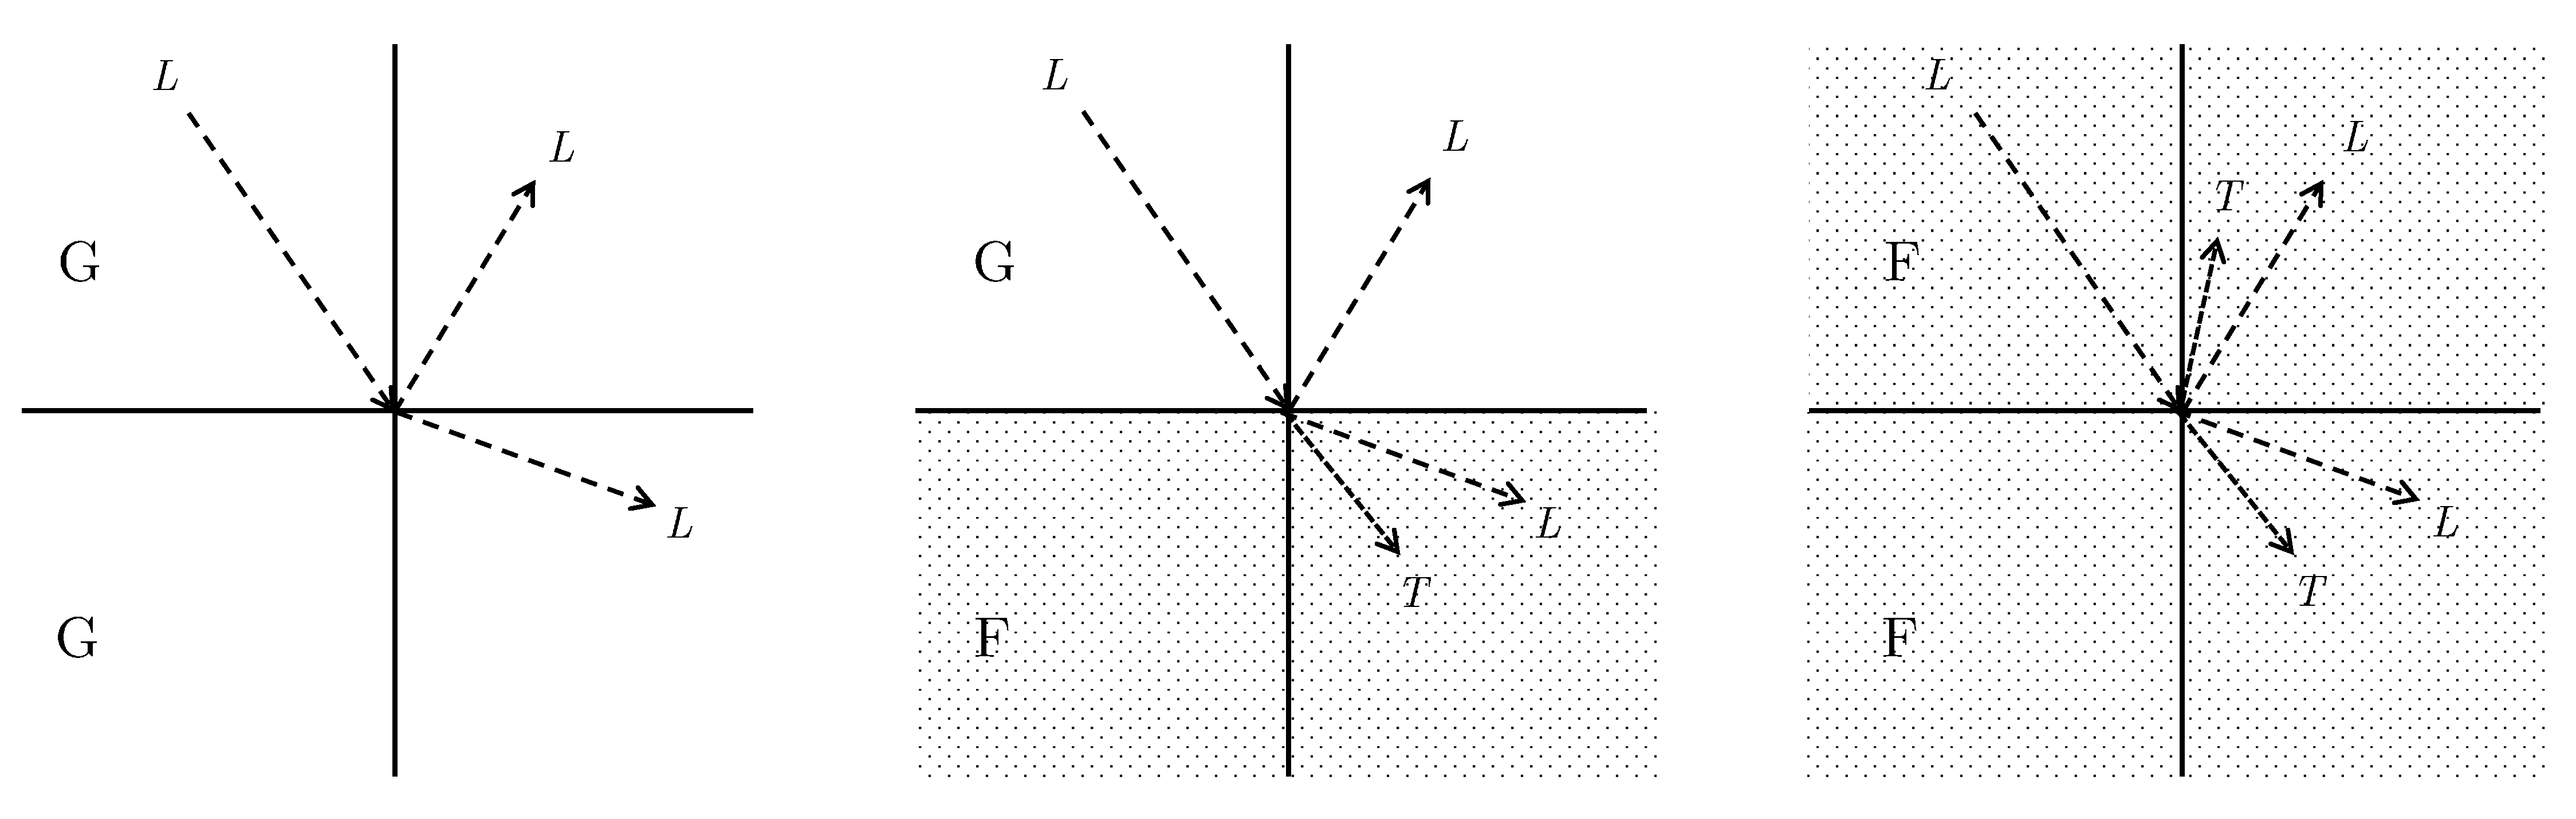
\includegraphics[width=\textwidth]{graphics/image_grundlagen_transmission_absorbtion.png}
\end{center}
\caption{Reflexion und Transmission von Schall beim Auftreffen auf Grenzflächen \cite{KOHLRAUSCH}} % picture caption
\label{fig:image_grundlagen_transmission_absorbtion}
\end{figure}
%
%(Abb. \ref{fig:image1})
%%%%%%%%%%%%%%%%%%%%%%%%%%%%%%%%%%%%%%%%%%%%%%%%%%%%%%%%%%%%%%%%%%%%%%%%%%%%%%%%

Dabei tritt beim Übergang in einen Festkörper sowohl eine Longitudinalwelle (L) als auch eine Transversalwelle (T) auf, die verschiedene Austrittswinkel aufweisen.


\subsubsection{Phased Array-Schallquellen}\label{sec:phased_array_schallquellen}
Anordnungen mehrerer Schallquellen nebeneinander werden als Array bezeichnet, dabei verändert sich die Richtcharakteristik des erzeugten Schalls. Es entsteht eine grosse Schallkeule, in welcher der Schalldruck am grössten ist, sowie mehrere Nebenkeulen.
Falls die einzelnen Schallquellen phasenverzögert angesteuert werden, lässt sich der Hauptkegel durch die verzögerte Ansteuerung drehen. Das Prinzip wird in Abbildung \ref{fig:image_grundlagen_phased_array} dargestellt.

%%%%%%%%%%%%%%%%%%%%%%%%%%%%%%%%%%%%%%%%%%%%%%%%%%%%%%%%%%%%%%%%%%%%%%%%%%%%%%%%
% pictures
\begin{figure}[htb]
\begin{center}
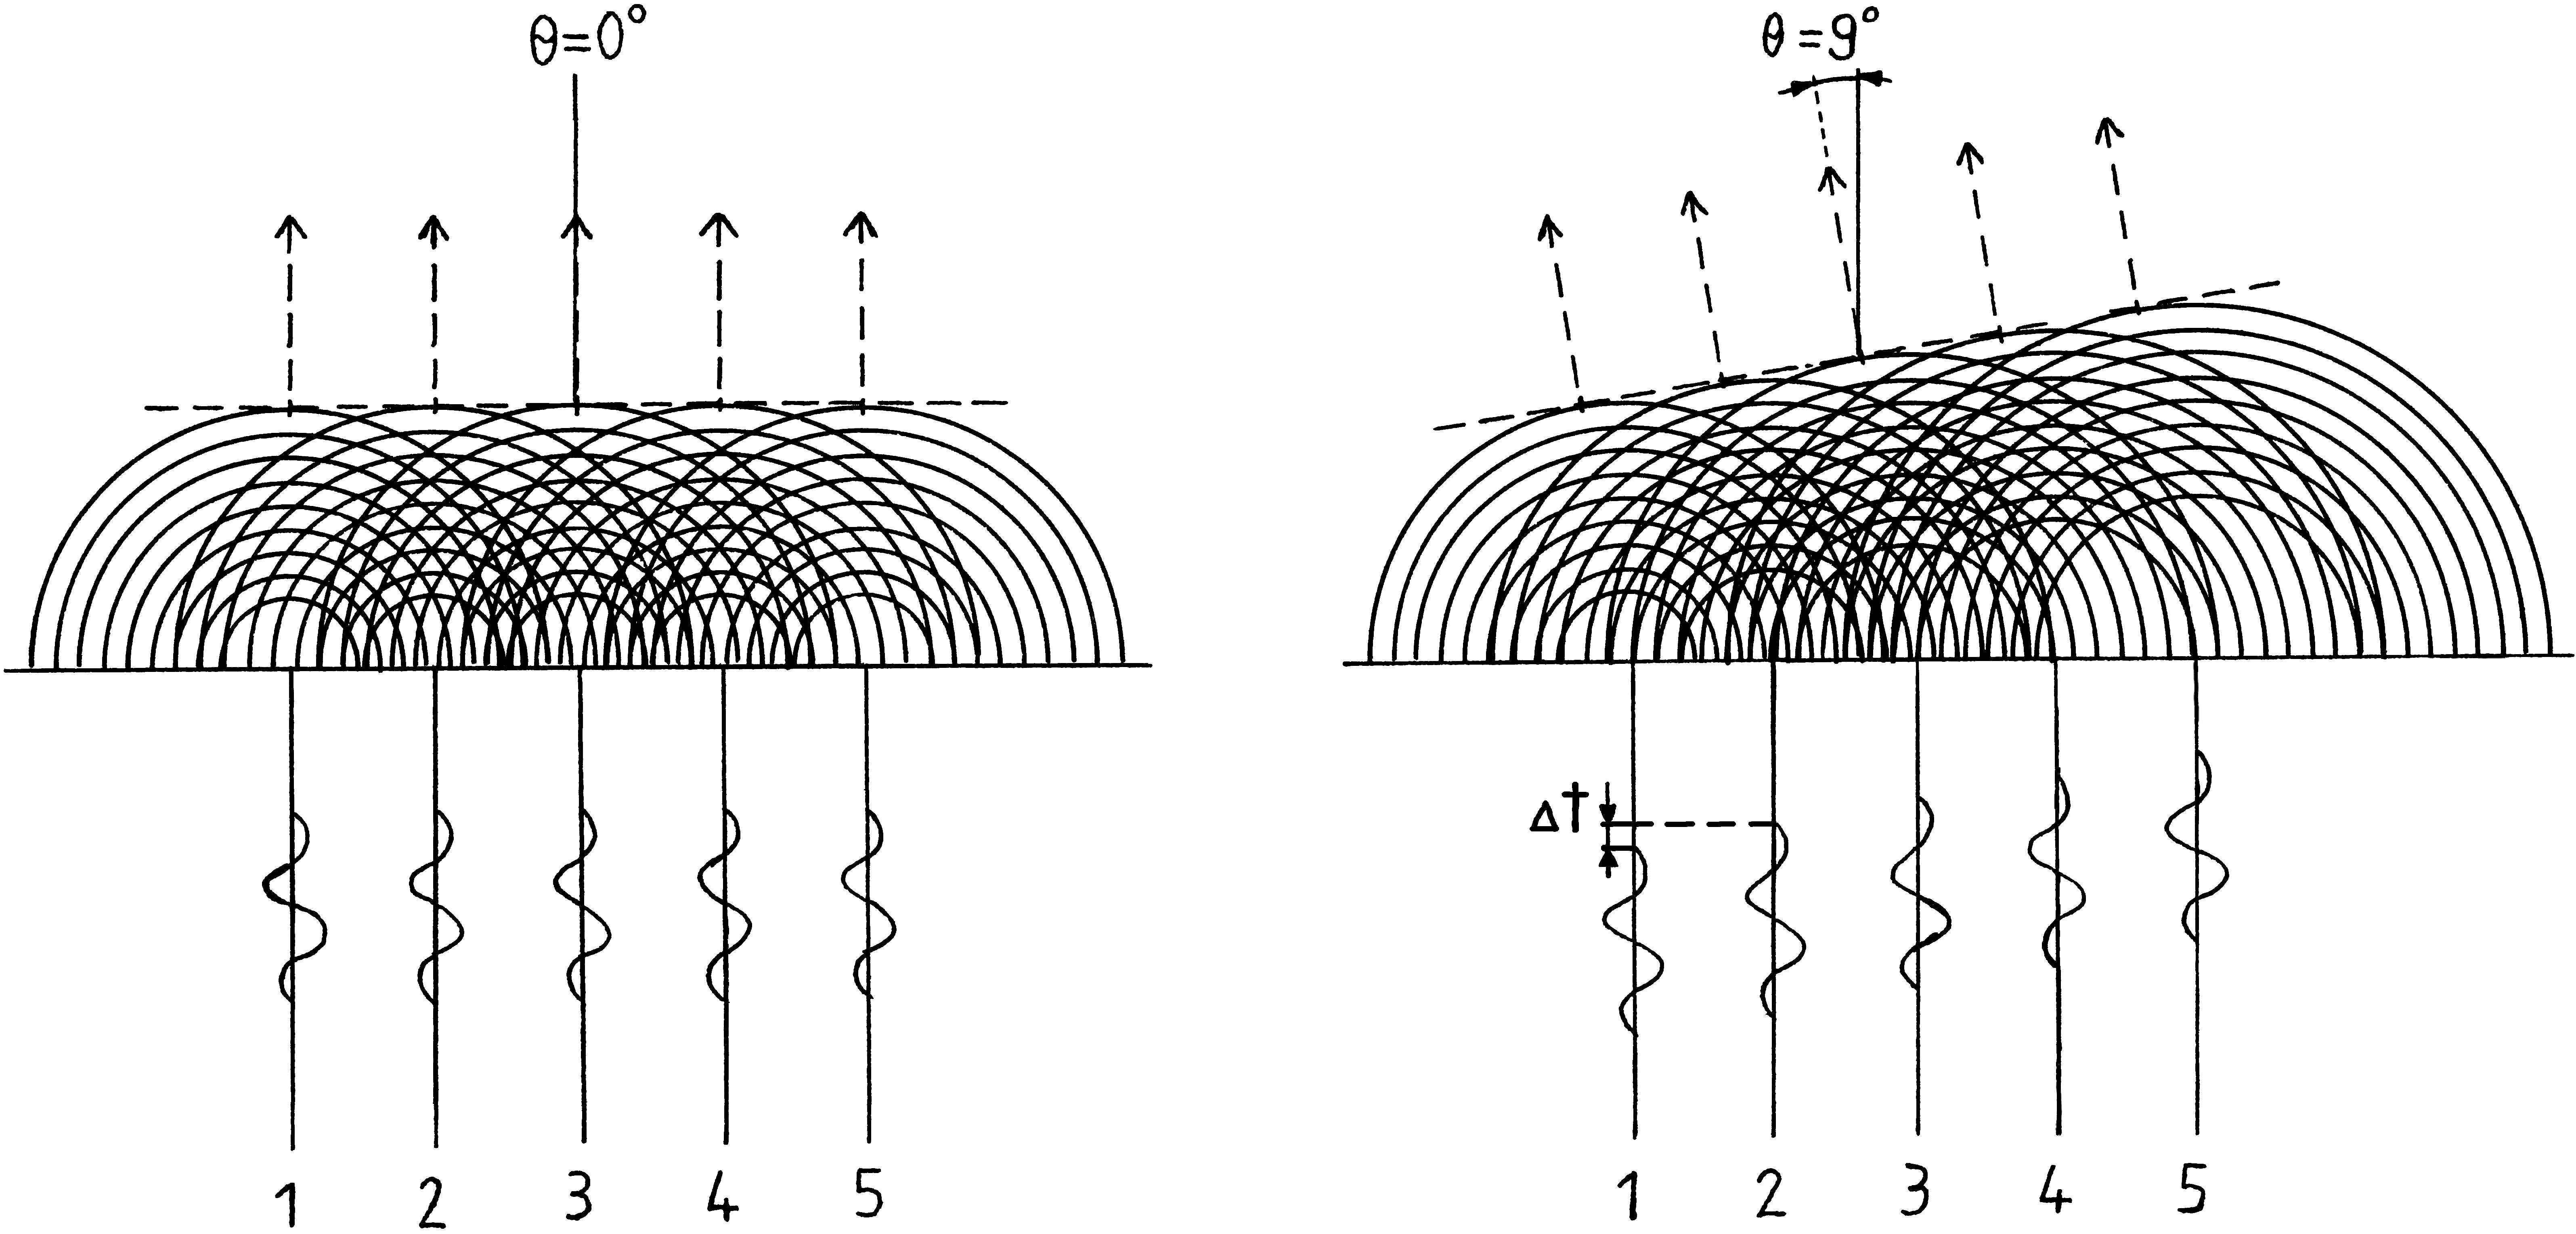
\includegraphics[width=\textwidth]{graphics/image_grundlagen_phased_array.png}
\end{center}
\caption{Prinzip eines linearen Phased Arrays, exemplarisch für 5 Kanäle} % picture caption
\label{fig:image_grundlagen_phased_array}
\end{figure}
%
%(Abb. \ref{fig:image1})
%%%%%%%%%%%%%%%%%%%%%%%%%%%%%%%%%%%%%%%%%%%%%%%%%%%%%%%%%%%%%%%%%%%%%%%%%%%%%%%%

Am häufigsten wird unterschieden zwischen linearen Arrays, bei denen die Elemente in einer Reihe angeordnet sind (siehe Abbildung \ref{fig:image_grundlagen_phased_array}), und planaren Arrays, bei denen die Schallquellen in einer Ebene liegen.

Die nötige Zeitverzögerung zwischen den Kanälen, um die Richtwirkung um den Winkel $\Theta$ zu erreichen, wird folgendermassen berechnet \cite{WOOH}:

%%%%%%%%%%%%%%%%%%%%%%%%%%%%%%%%%%%%%%%%%%%%%%%%%%%%%%%%%%%%%%%%%%%%%%%%%%%%%%%%
\begin{equation}
\Delta \tau = \frac{d \cdot \sin(\Theta )}{c}
\label{eq:zeitverzögerung_winkel}
\end{equation}
%%%%%%%%%%%%%%%%%%%%%%%%%%%%%%%%%%%%%%%%%%%%%%%%%%%%%%%%%%%%%%%%%%%%%%%%%%%%%%%%

In (\ref{eq:zeitverzögerung_winkel}) bezeichnet $c$ die Schallgeschwindigkeit und $d$ den Abstand zwischen den Elementen des Phased Arrays.

Der Schalldruck im Fernfeld eines linearen Phased Arrays ($r \gg d$) in Abhängigkeit des Winkels, der Distanz und der Zeit lässt sich nach dem huygensschen Prinzip berechnen, dessen Herleitung in \cite{SKUDRZYK} zu finden ist. Für dieses Projekt interessant ist die Richtcharakteristik. Gemäss \cite{WOOH} ergibt sich nach einer Normierung auf den Schalldruck in Richtung des Sendewinkels folgende Beziehung zwischen dem Betrag des normierten Schalldrucks $H(\varphi)$ und dem Winkel $\varphi$, in dem man zum Array steht:

%%%%%%%%%%%%%%%%%%%%%%%%%%%%%%%%%%%%%%%%%%%%%%%%%%%%%%%%%%%%%%%%%%%%%%%%%%%%%%%%
\begin{equation}
 H(\varphi ) = \left | \frac{\sin(  \frac{\pi \cdot d \cdot (\sin(\theta)-\sin(\varphi))}{\lambda}\cdot N)}{\sin(\frac{\pi \cdot d \cdot (\sin(\theta)-\sin(\varphi))}{\lambda})} \right |
\label{eq:richtcharakteristik}
\end{equation}
%%%%%%%%%%%%%%%%%%%%%%%%%%%%%%%%%%%%%%%%%%%%%%%%%%%%%%%%%%%%%%%%%%%%%%%%%%%%%%%%

In (\ref{eq:richtcharakteristik}) bezeichnet $\theta$ den durch Phasenverzögerung eingestellten Sendewinkel, $\lambda$ die Wellenlänge, $d$ den Abstand zwischen den Sensoren und $N$ die Anzahl Elemente im Array. Ausgewertet für eine steigende Anzahl Elemente $N$ im Array und für verschiedene Abstände $d$ zwischen den Schallquellen ergeben sich die Abbildungen \ref{fig:plot_grundlagen_characteristic_calc_0} und \ref{fig:plot_grundlagen_characteristic_calc_1}.

%%%%%%%%%%%%%%%%%%%%%%%%%%%%%%%%%%%%%%%%%%%%%%%%%%%%%%%%%%%%%%%%%%%%%%%%%%%%%%%%
% pictures
\begin{figure}[htb]
\begin{center}
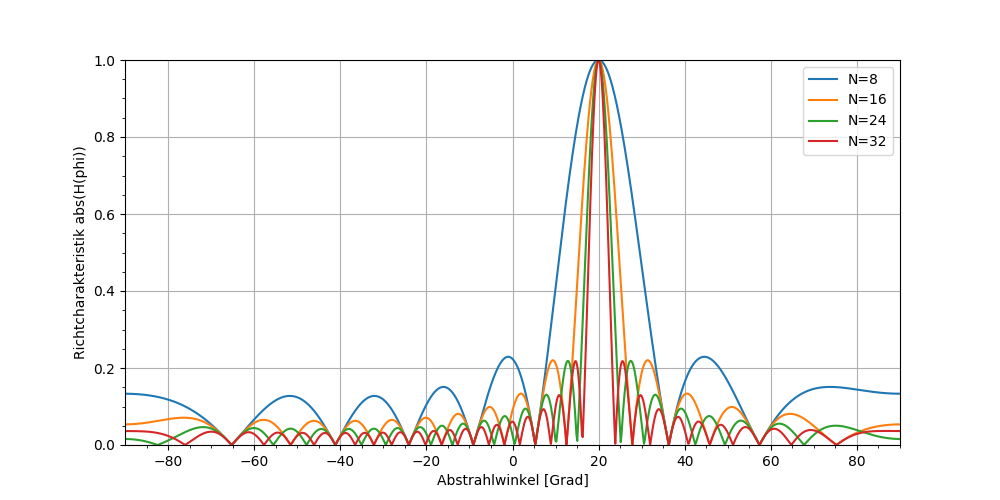
\includegraphics[width=\textwidth]{graphics/plot_grundlagen_characteristic_calc_0.png}
\end{center}
\caption{Richtcharakteristik für eine unterschiedliche Anzahl Elemente bei einem Abstand $d = \lambda /2$ und einem Sendewinkel von 20 Grad} % picture caption
\label{fig:plot_grundlagen_characteristic_calc_0}
%\end{figure}
%
%(Abb. \ref{fig:image1})
%%%%%%%%%%%%%%%%%%%%%%%%%%%%%%%%%%%%%%%%%%%%%%%%%%%%%%%%%%%%%%%%%%%%%%%%%%%%%%%%

%%%%%%%%%%%%%%%%%%%%%%%%%%%%%%%%%%%%%%%%%%%%%%%%%%%%%%%%%%%%%%%%%%%%%%%%%%%%%%%%
% pictures
%\begin{figure}[htb]
\begin{center}
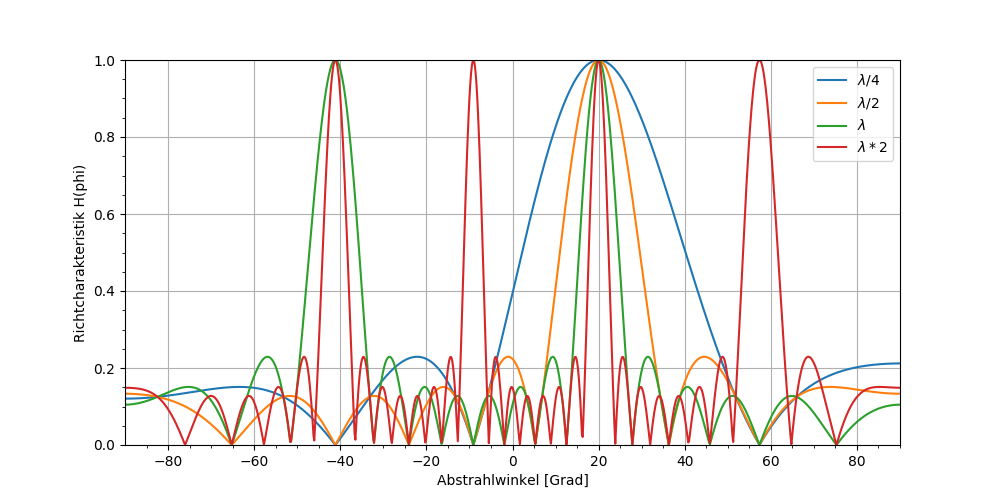
\includegraphics[width=\textwidth]{graphics/plot_grundlagen_characteristic_calc_1.png}
\end{center}
\caption{Richtcharakteristik für verschiedene Abstände bei $N = 8$ Elementen und einem Sendewinkel von 20 Grad} % picture caption
\label{fig:plot_grundlagen_characteristic_calc_1}
\end{figure}
%
%(Abb. \ref{fig:image1})
%%%%%%%%%%%%%%%%%%%%%%%%%%%%%%%%%%%%%%%%%%%%%%%%%%%%%%%%%%%%%%%%%%%%%%%%%%%%%%%%

Wird die Anzahl Elemente $N$ erhöht, so entsteht eine schmalere Hauptkeule und mehrere Seitenkeulen (siehe Abbildung \ref{fig:plot_grundlagen_characteristic_calc_0}). Ist der Abstand zwischen den Elementen grösser als die Wellenlänge $\lambda$, so entstehen viele Seitenkeulen, wovon einzelne gleich gross sind wie die Hauptkeule. Für Abstände kleiner als $\lambda$ verschwinden diese grossen Nebenkeulen, jedoch nimmt die Breite der Hauptkeulen zu (siehe Abbildung \ref{fig:plot_grundlagen_characteristic_calc_1}).

Es kann zusätzlich ein Schärfefaktor $q$ berechnet werden, der beschreibt, wie stark gerichtet die Hauptkeule ist \cite{WOOH}:

%%%%%%%%%%%%%%%%%%%%%%%%%%%%%%%%%%%%%%%%%%%%%%%%%%%%%%%%%%%%%%%%%%%%%%%%%%%%%%%%
\begin{equation}
q = \frac{1}{\pi} \cdot \left [  \sin^{^{-1}}(\sin(\theta)+\frac{\lambda}{N \cdot d})-\sin^{^{-1}}(\sin(\theta)-\frac{\lambda}{N \cdot d}) \right ]
\label{eq:schaerfefaktor}
\end{equation}
%%%%%%%%%%%%%%%%%%%%%%%%%%%%%%%%%%%%%%%%%%%%%%%%%%%%%%%%%%%%%%%%%%%%%%%%%%%%%%%%

Ein kleineres $q$ bedeutet eine steilere Hauptkeule. Ausgewertet für eine variierende Anzahl Elemente $N$ und verschiedene Sendewinkel $\theta$ sowie für die im Projekt verwendete Frequenz von $40 \mathrm{kHz}$ und einen Abstand von $d = 5.4 \mathrm{mm}$ entstehen die Abbildungen \ref{fig:plot_grundlagen_sharpness_factor_calc_0} und \ref{fig:plot_grundlagen_sharpness_factor_calc_1}.

%%%%%%%%%%%%%%%%%%%%%%%%%%%%%%%%%%%%%%%%%%%%%%%%%%%%%%%%%%%%%%%%%%%%%%%%%%%%%%%%
% pictures
\begin{figure}[htb]
\begin{center}
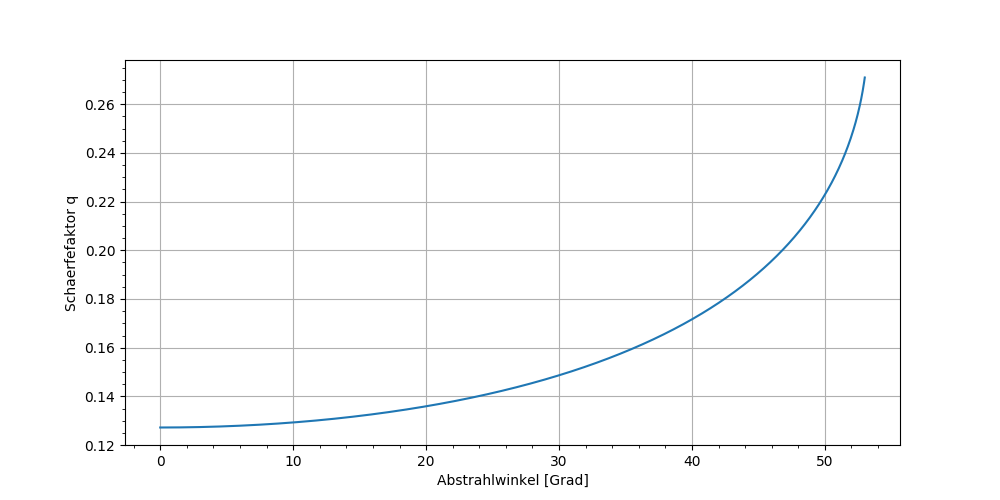
\includegraphics[width=\textwidth]{graphics/plot_grundlagen_sharpness_factor_calc_0.png}
\end{center}
\caption{Schärfefaktor für unterschiedliche Abstrahlwinkel, $N = 8$} % picture caption
\label{fig:plot_grundlagen_sharpness_factor_calc_0}
%\end{figure}
%
%(Abb. \ref{fig:image1})
%%%%%%%%%%%%%%%%%%%%%%%%%%%%%%%%%%%%%%%%%%%%%%%%%%%%%%%%%%%%%%%%%%%%%%%%%%%%%%%%

%%%%%%%%%%%%%%%%%%%%%%%%%%%%%%%%%%%%%%%%%%%%%%%%%%%%%%%%%%%%%%%%%%%%%%%%%%%%%%%%
% pictures
%\begin{figure}[htb]
\begin{center}
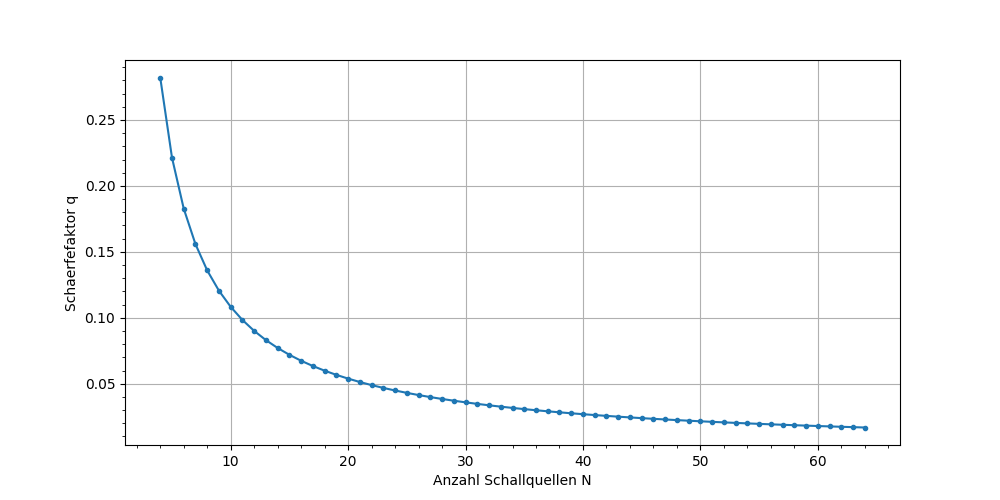
\includegraphics[width=\textwidth]{graphics/plot_grundlagen_sharpness_factor_calc_1.png}
\end{center}
\caption{Schärfefaktor für eine steigende Anzahl Elemente bei einem Abstrahlwinkel von 20 Grad} % picture caption
\label{fig:plot_grundlagen_sharpness_factor_calc_1}
\end{figure}
%
%(Abb. \ref{fig:image1})
%%%%%%%%%%%%%%%%%%%%%%%%%%%%%%%%%%%%%%%%%%%%%%%%%%%%%%%%%%%%%%%%%%%%%%%%%%%%%%%%

Je grösser der Sendewinkel ist, desto weniger steil wird die Hauptkeule. Mit einer grösseren Anzahl Elemente $N$ kann $q$ theoretisch unendlich klein werden. Den gleichen Effekt hätte eine kleinere Wellenlänge $\lambda$ bei gleichbleibendem Abstand $d$ oder umgekehrt eine Vergrösserung des Abstands. Dies ist jedoch nicht wünschenswert, weil dadurch grosse Nebenkeulen entstehen. Diese sind in Abbildung \ref{fig:plot_grundlagen_characteristic_calc_1} dargestellt.


\clearpage
\subsubsection{Simulationen}\label{sec:simulationen}
Die für das Projekt verwendeten Dimensionen (siehe Kapitel \ref{sec:hardware}) werden mit der Opensource-Toolbox k-Wave simuliert. Dabei wird nun im Gegensatz zu den obigen Berechnungen auch das Nahfeld berücksichtigt. Als Schallquellen werden acht ideale Punktquellen verwendet, die ein Wellenpaket bestehend aus 25 Schwingungen aussenden. In den Abbildungen \ref{fig:image_grundlagen_sim_0_degrees}, \ref{fig:image_grundlagen_sim_10_degrees} und \ref{fig:image_grundlagen_sim_20_degrees} wird das Maximum des Schalldrucks auf $1 \mathrm{m}$ Distanz für verschiedene Abstrahlwinkel dargestellt.

\begin{figure}[hb]
\begin{minipage}{0.5\textwidth}
%%%%%%%%%%%%%%%%%%%%%%%%%%%%%%%%%%%%%%%%%%%%%%%%%%%%%%%%%%%%%%%%%%%%%%%%%%%%%%%%
% pictures
%\begin{figure}[htb]
\begin{center}
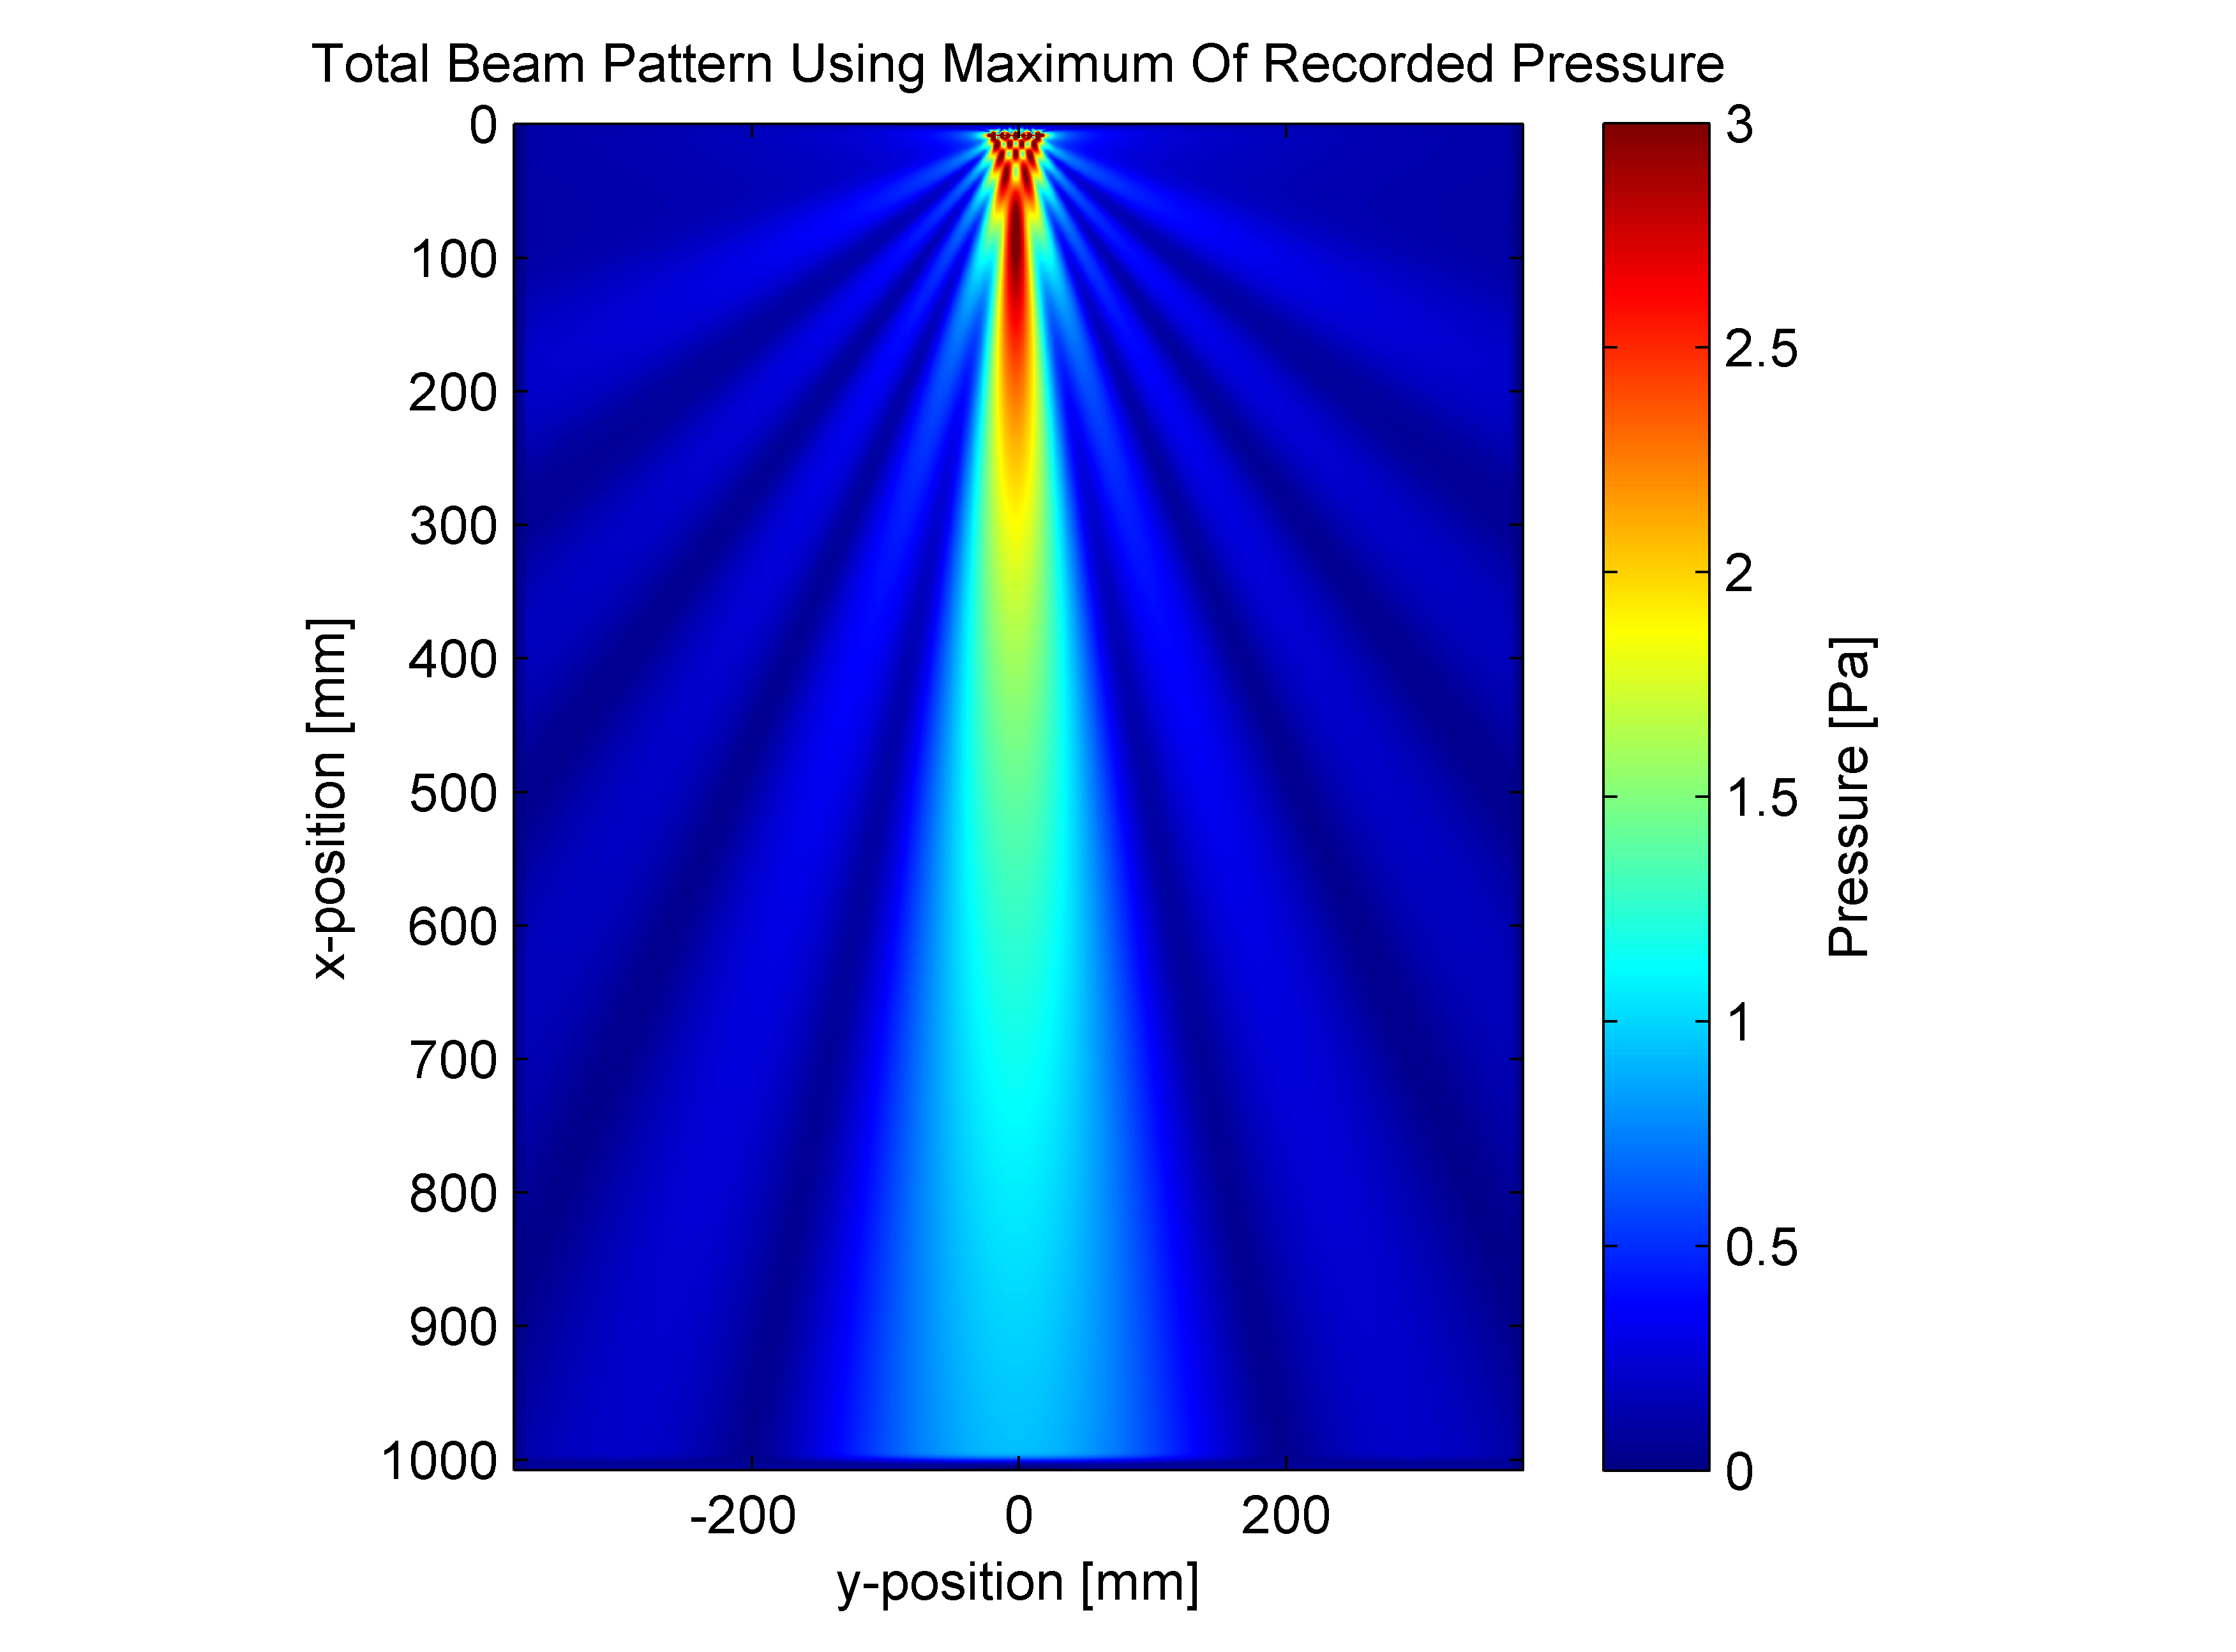
\includegraphics[width=1.2\textwidth]{graphics/image_grundlagen_sim_0_degrees.png}
\end{center}
\caption{Simulation für $N = 8$, $d = 5.4 \mathrm{mm}$, bei einer Frequenz von $40 \mathrm{kHz}$ in Luft für einen Sendewinkel von 0 Grad} % picture caption
\label{fig:image_grundlagen_sim_0_degrees}
%\end{figure}
%
%(Abb. \ref{fig:image1})
%%%%%%%%%%%%%%%%%%%%%%%%%%%%%%%%%%%%%%%%%%%%%%%%%%%%%%%%%%%%%%%%%%%%%%%%%%%%%%%%
\end{minipage}
\begin{minipage}{0.5\textwidth}
%%%%%%%%%%%%%%%%%%%%%%%%%%%%%%%%%%%%%%%%%%%%%%%%%%%%%%%%%%%%%%%%%%%%%%%%%%%%%%%%
% pictures
%\begin{figure}[htb]
\begin{center}
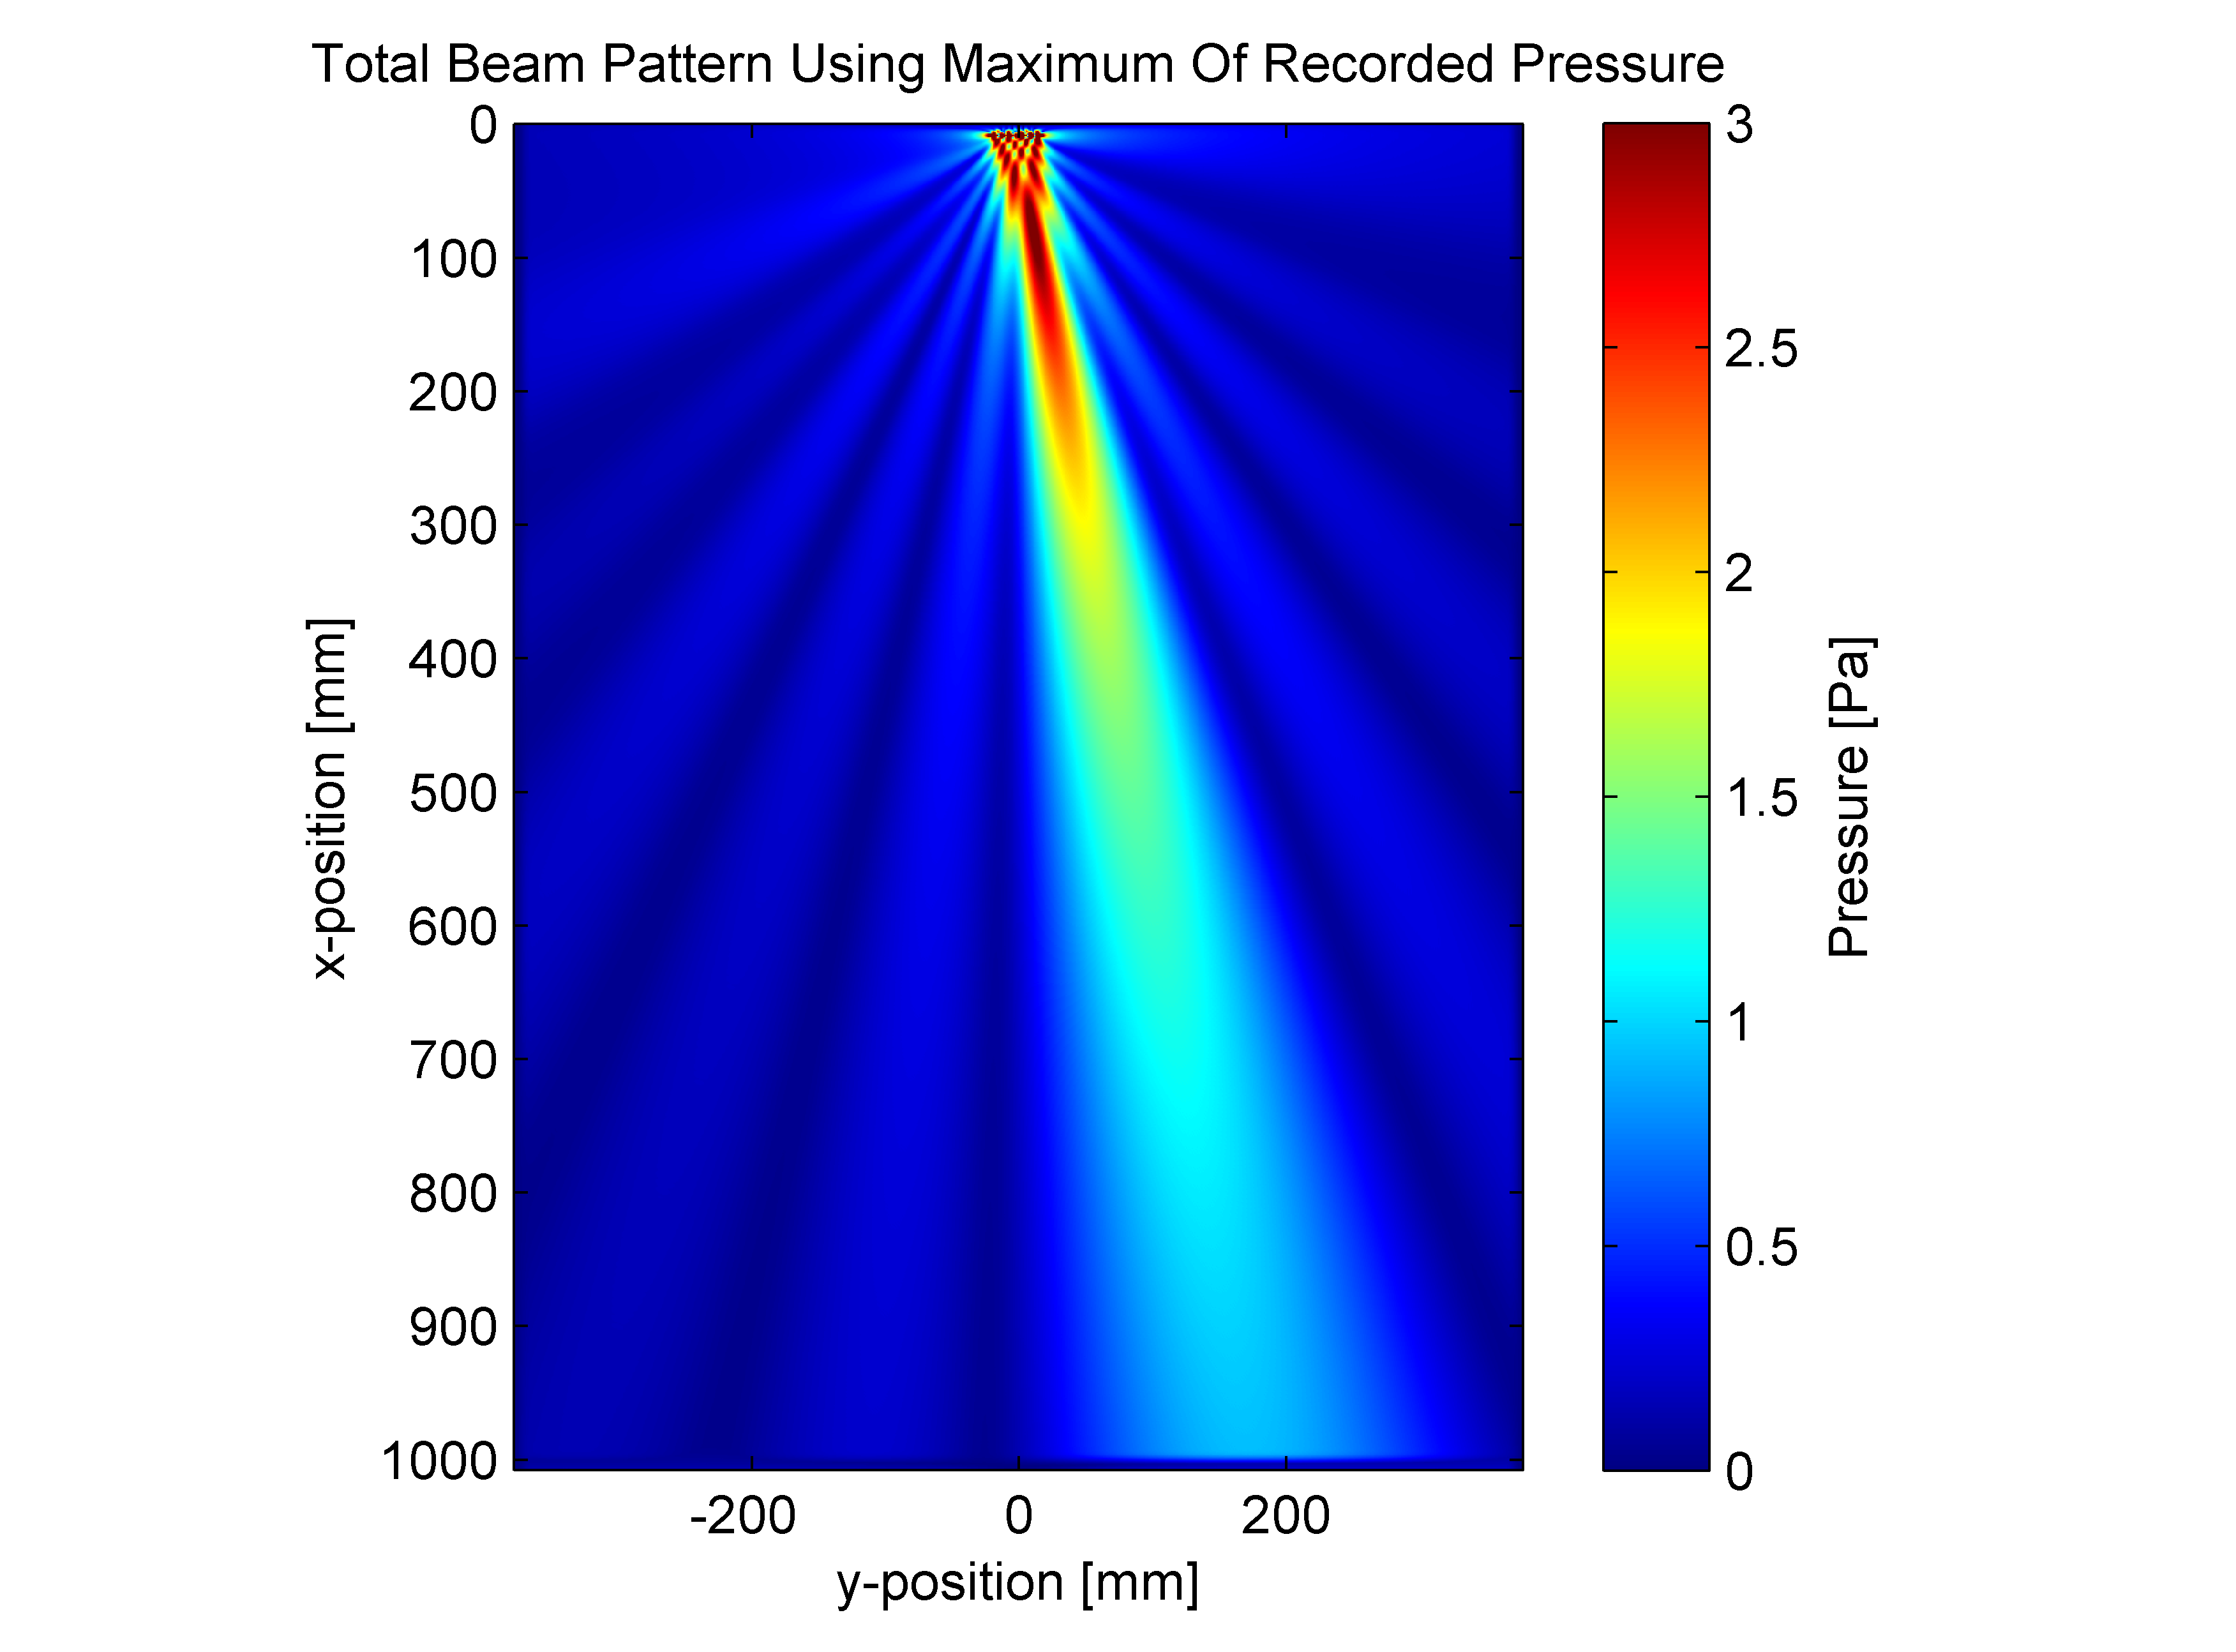
\includegraphics[width=1.2\textwidth]{graphics/image_grundlagen_sim_10_degrees.png}
\end{center}
\caption{Simulation für $N = 8$, $d = 5.4 \mathrm{mm}$, bei einer Frequenz von $40 \mathrm{kHz}$ in Luft für einen Sendewinkel von 10 Grad} % picture caption
\label{fig:image_grundlagen_sim_10_degrees}
%\end{figure}
%
%(Abb. \ref{fig:image1})
%%%%%%%%%%%%%%%%%%%%%%%%%%%%%%%%%%%%%%%%%%%%%%%%%%%%%%%%%%%%%%%%%%%%%%%%%%%%%%%%
\end{minipage}
\begin{minipage}{0.5\textwidth}
%%%%%%%%%%%%%%%%%%%%%%%%%%%%%%%%%%%%%%%%%%%%%%%%%%%%%%%%%%%%%%%%%%%%%%%%%%%%%%%%
% pictures
%\begin{figure}[htb]
\begin{center}
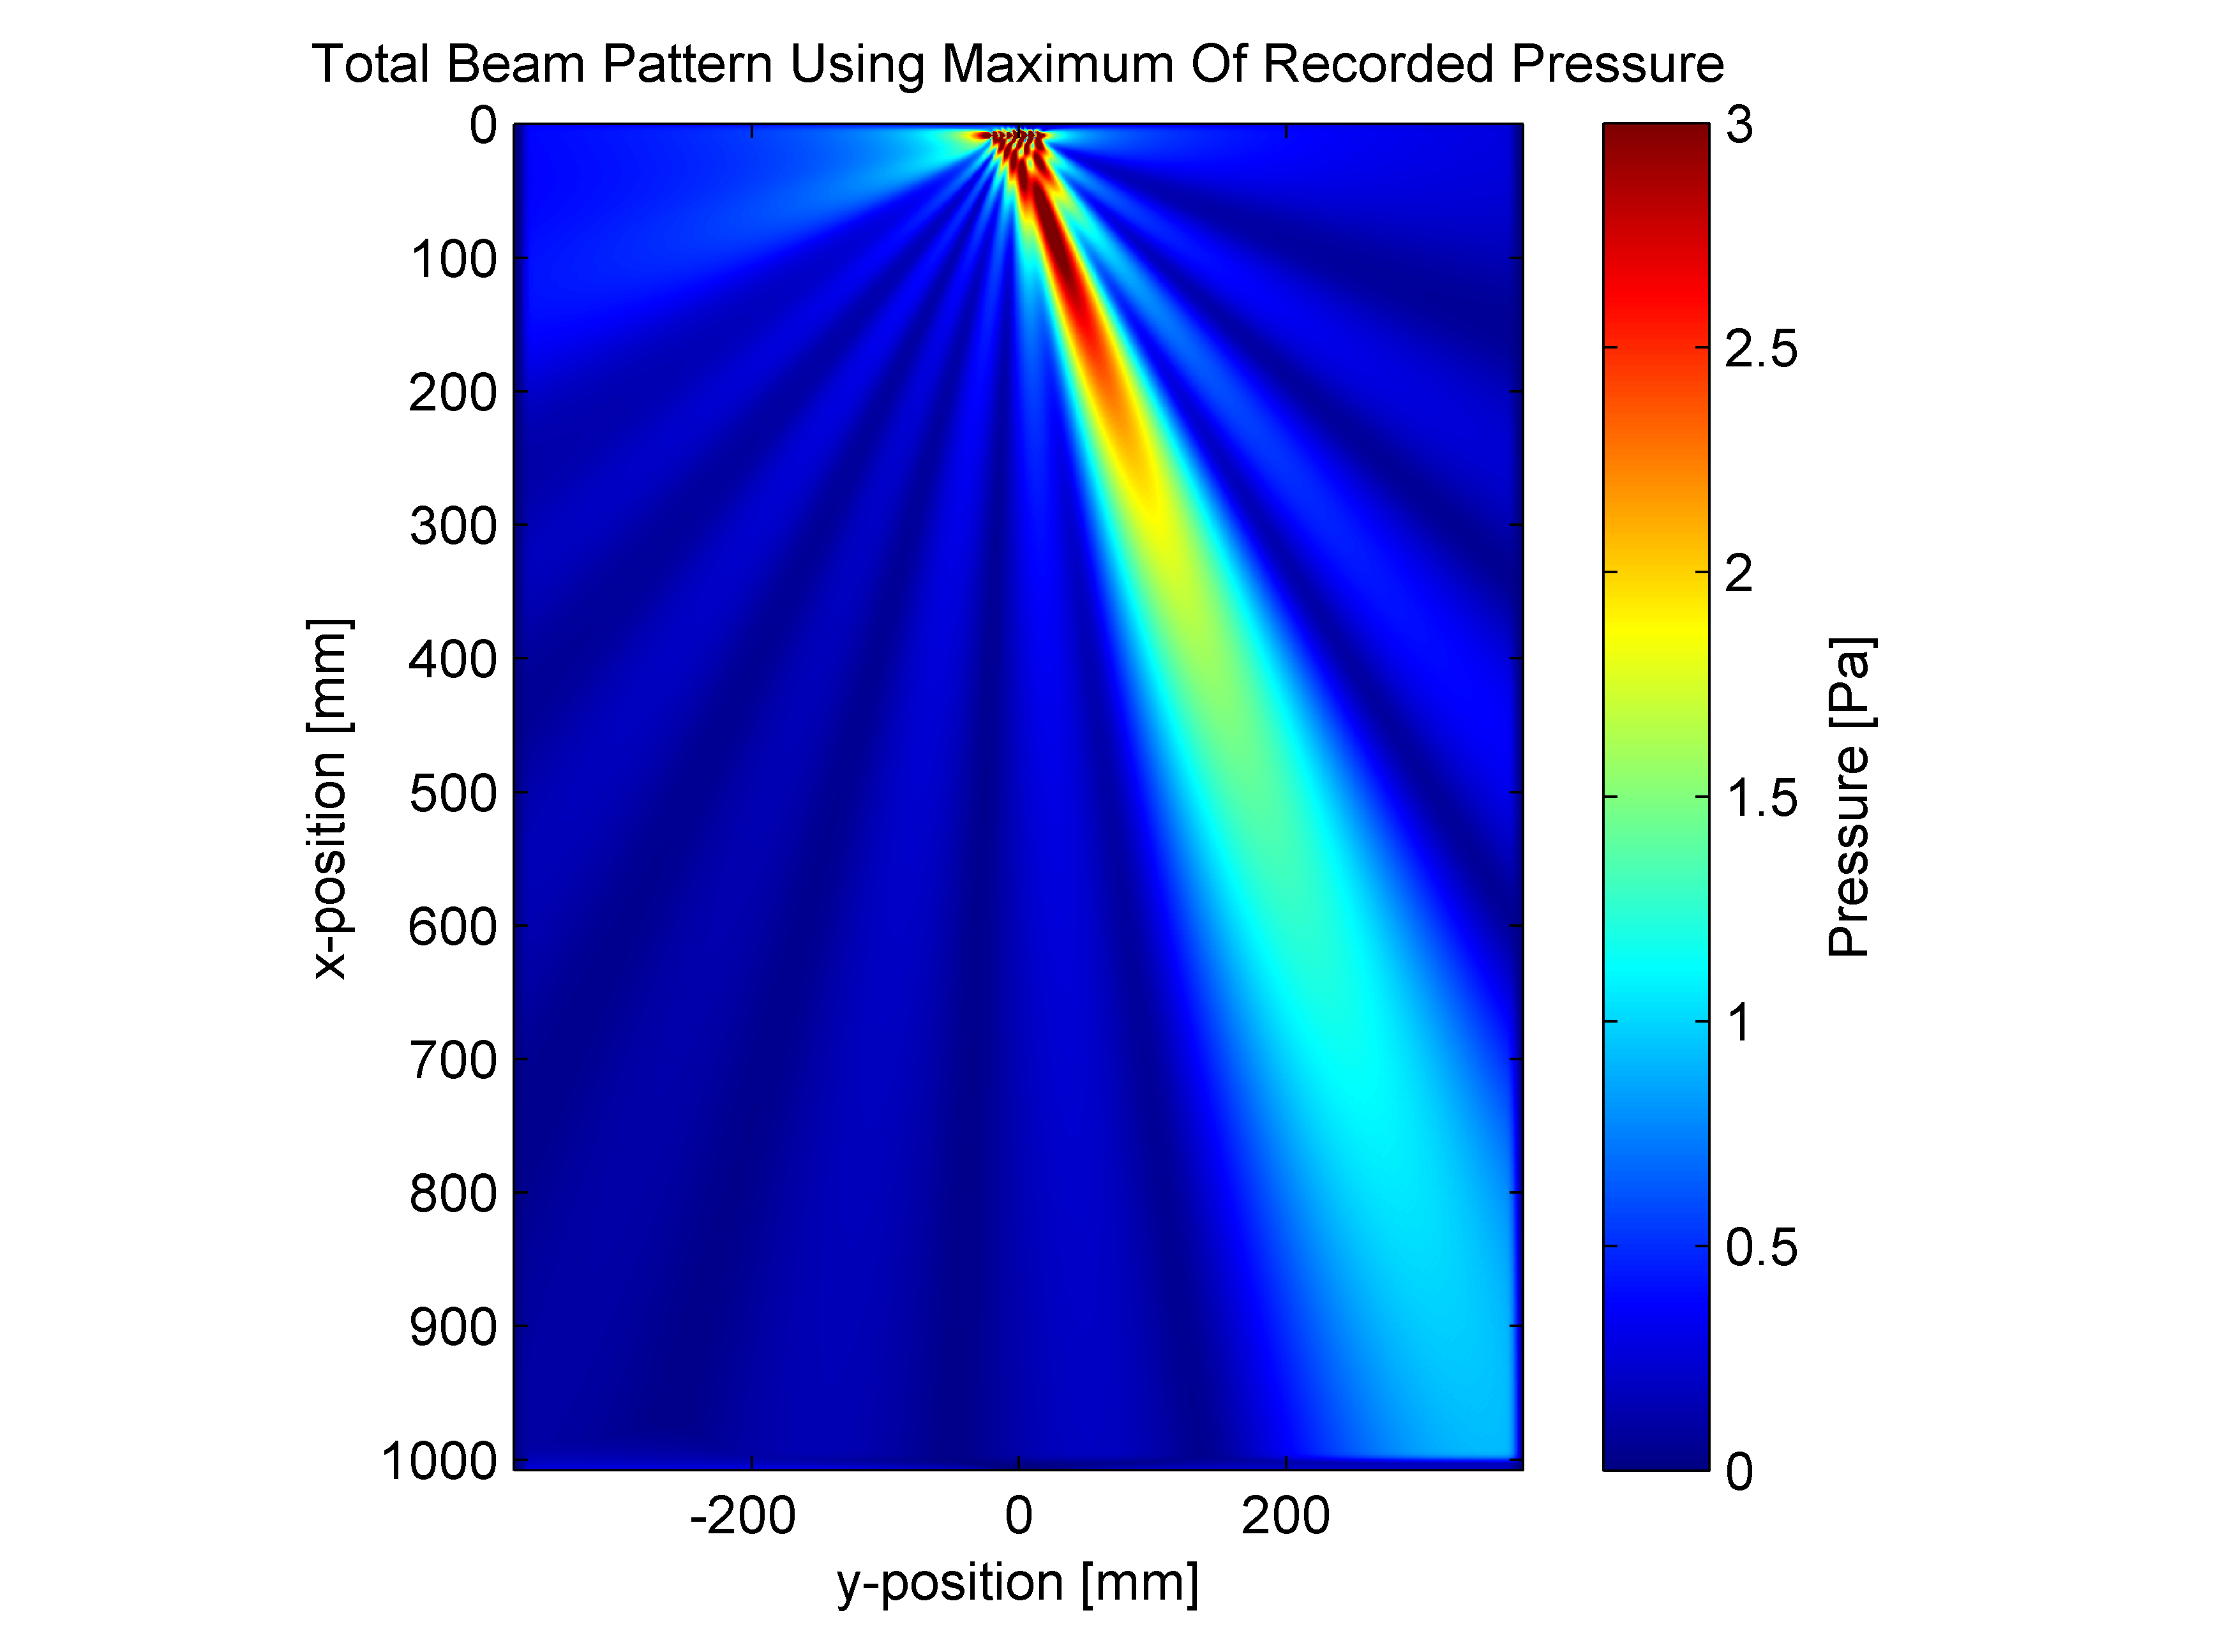
\includegraphics[width=1.2\textwidth]{graphics/image_grundlagen_sim_20_degrees.png}
\end{center}
\caption{Simulation für $N = 8$, $d = 5.4 \mathrm{mm}$, bei einer Frequenz von $40 \mathrm{kHz}$ in Luft für einen Sendewinkel von 20 Grad} % picture caption
\label{fig:image_grundlagen_sim_20_degrees}
%\end{figure}
%
%(Abb. \ref{fig:image1})
%%%%%%%%%%%%%%%%%%%%%%%%%%%%%%%%%%%%%%%%%%%%%%%%%%%%%%%%%%%%%%%%%%%%%%%%%%%%%%%%
\end{minipage}
\end{figure}


\clearpage
\subsubsection{Amplitudenbelegung}\label{sec:amplitudenbelegung}
Aus der Abbildung \ref{fig:plot_grundlagen_characteristic_calc_0} im Kapitel \ref{sec:phased_array_schallquellen} ist ersichtlich, dass durch die Erhöhung der Anzahl Elemente zwar die Hauptkeule und die Nebenkeulen schmaler werden und näher zusammenrücken, man sieht aber auch, dass sich die Intensität der Nebenkeulen nur gering verändert. Auch das Verhältnis zwischen dem Abstand der Elemente und der Wellenlänge haben, wie in Abbildung \ref{fig:plot_grundlagen_characteristic_calc_1} im Kapitel \ref{sec:phased_array_schallquellen} zu sehen ist, keinen grossen Einfluss auf die Intensität der Nebenkeulen. Will man die Nebenkeulen stärker dämpfen, kann dies durch eine Amplitudenbelegung der einzelnen Elemente erreicht werden. Dabei wird nicht jedes Element mit derselben Amplitude angesteuert, sondern von aussen nach innen symmetrisch mit unterschiedlichen Amplituden. Die Idee dazu stammt aus der Hochfrequenztechnik, wo Phased Array-Antennen zur Erzeugung einer starken Richtwirkung, zum Beispiel bei Datenübertragungs- oder Radarsystemen, eingesetzt werden. Die entsprechende Theorie stammt aus den Quellen \cite{ELECTROMAGNETICS} und \cite{VISSER}.

Weisen alle Elemente dieselbe Amplitude auf, spricht man von einer Rechteckbelegung. Die resultierende Richtcharakteristik weist bei dieser Belegung eine $\sin(x)/x$-förmige Intensitätsverteilung auf. Dies legt die Vermutung nahe, dass die Amplitudenbelegung und die Intensitätsverteilung der Richtcharakteristik über die Fouriertransformation zusammenhängen. Diese Vermutung wird durch \cite{ELECTROMAGNETICS} bestätigt, wo sich auch gleich eine Anzahl üblicher Belegungsfunktionen findet, mit welchen die Nebenkeulen gut gedämpft werden können. In den Abbildungen \ref{fig:plot_grundlagen_characteristic_calc_aperture} und \ref{fig:plot_grundlagen_characteristic_calc_aperture_log} ist die Richtcharakteristik für vier verschiedene Amplitudenbelegungen dargestellt, im ersten Bild mit linearer Skalierung und normiert auf eins, in der zweiten Abbildung logarithmisch. Die Anzahl Elemente und der Abstand dazwischen entsprechen der in diesem Projekt entwickelten Hardware.

Da das Prinzip der Phased Array-Antennen auf konstruktiver und destruktiver Interferenz beruht, werden zur Berechnung die Anteile der einzelnen Strahler mit der Belegungsfunktion gewichtet und aufsummiert. Die Formel dazu lautet wie folgt \cite{VISSER}:

%%%%%%%%%%%%%%%%%%%%%%%%%%%%%%%%%%%%%%%%%%%%%%%%%%%%%%%%%%%%%%%%%%%%%%%%%%%%%%%%
\begin{equation}
\left | \underline{H}(\varphi) \right | = \left | \sum\limits_{i = 1}^{N}{A_{i} \cdot e^{\frac{j 2 \pi d}{\lambda} \cdot (N - i) \cdot (\sin{(\phi_{0})} - \sin{(\phi)})}} \right |
\label{eq:amplitudenbelegung}
\end{equation}
%%%%%%%%%%%%%%%%%%%%%%%%%%%%%%%%%%%%%%%%%%%%%%%%%%%%%%%%%%%%%%%%%%%%%%%%%%%%%%%%

Dabei ist $N$ die Anzahl Elemente, $d$ der Abstand zwischen den Elementen, $\lambda$ die Wellenlänge, $A_{i}$ der Gewichtungsfaktor der Amplitudenbelegung und $\phi_{0}$ der eingestellte Sendewinkel. Für eine Rechteckbelegung ($A_{i} = 1$) lässt sich diese Formel umformen zur Formel \ref{eq:richtcharakteristik} aus dem Kapitel \ref{sec:phased_array_schallquellen}.

In den Abbildungen \ref{fig:plot_grundlagen_characteristic_calc_aperture} und \ref{fig:plot_grundlagen_characteristic_calc_aperture_log} ist gut zu sehen, dass eine bessere Nebenkeulenunterdrückung gleichzeitig in einer breiteren Hauptkeule resultiert. Dies könnte nun wiederum durch eine grössere Anzahl Elemente kompensiert werden. Die Rechteckbelegung weist zwar eine sehr schmale Hauptkeule auf, die ersten Nebenkeulen sind aber um lediglich etwas mehr als $12 \mathrm{dB}$ gedämpft. Mit einer $\cos$-förmigen Belegung kann die erste Hauptkeule bereits um ca. $18 \mathrm{dB}$ gedämpft werden, mit einer $\cos^{2}$-Belegung um etwa $26 \mathrm{dB}$ und mit einer Gaussbelegung um mehr als $30 \mathrm{dB}$. Diese bessere Nebenkeulenunterdrückung erkauft man sich im Falle der Gaussbelegung mit einer ungefähr $1.5$ Mal breiteren Hauptkeule als bei einer Rechteckbelegung, bezogen auf den $3 \mathrm{dB}$-Öffnungswinkel.

Neben der Amplitudenbelegung hat auch die Richtcharakteristik der einzelnen Elemente einen Einfluss auf die Richtcharakteristik des ganzen Phased Arrays. Die resultierende Gesamtcharakteristik ist das Produkt aus der berechneten Richtcharakteristik des Arrays (mit Amplitudenbelegung) und der Richtcharakteristik eines einzelnen Elements.

\clearpage

%%%%%%%%%%%%%%%%%%%%%%%%%%%%%%%%%%%%%%%%%%%%%%%%%%%%%%%%%%%%%%%%%%%%%%%%%%%%%%%%
% pictures
\begin{figure}[htb]
\begin{center}
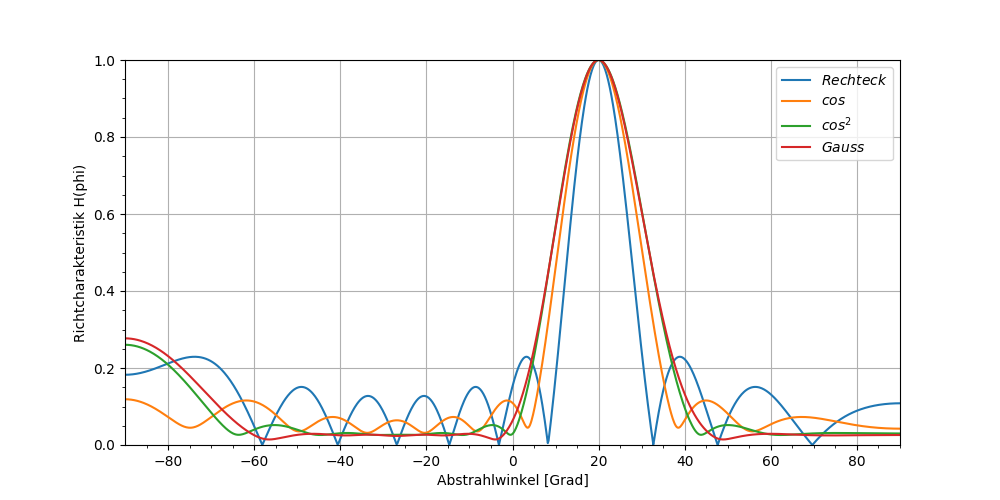
\includegraphics[width=\textwidth]{graphics/plot_grundlagen_characteristic_calc_aperture.png}
\end{center}
\caption{Richtcharakteristik für $N = 8$, $d = 5.4 \mathrm{mm}$ und einem Sendewinkel von 20 Grad} % picture caption
\label{fig:plot_grundlagen_characteristic_calc_aperture}
\end{figure}
%
%(Abb. \ref{fig:image1})
%%%%%%%%%%%%%%%%%%%%%%%%%%%%%%%%%%%%%%%%%%%%%%%%%%%%%%%%%%%%%%%%%%%%%%%%%%%%%%%%

%%%%%%%%%%%%%%%%%%%%%%%%%%%%%%%%%%%%%%%%%%%%%%%%%%%%%%%%%%%%%%%%%%%%%%%%%%%%%%%%
% pictures
\begin{figure}[htb]
\begin{center}
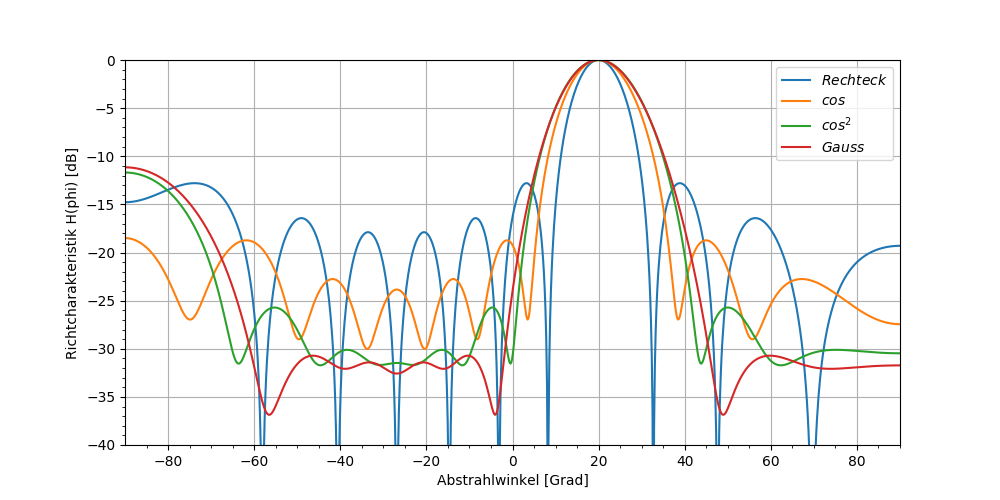
\includegraphics[width=\textwidth]{graphics/plot_grundlagen_characteristic_calc_aperture_log.png}
\end{center}
\caption{Richtcharakteristik für $N = 8$, $d = 5.4 \mathrm{mm}$ und einem Sendewinkel von 20 Grad} % picture caption
\label{fig:plot_grundlagen_characteristic_calc_aperture_log}
\end{figure}
%
%(Abb. \ref{fig:image1})
%%%%%%%%%%%%%%%%%%%%%%%%%%%%%%%%%%%%%%%%%%%%%%%%%%%%%%%%%%%%%%%%%%%%%%%%%%%%%%%%


\subsubsection{Phased Array-Sensoren}\label{sec:phased_array_sensoren}
Die Theorie für Arrays aus Schallquellen ist praktisch identisch für Arrays aus Empfängern. Ein schräg auf das Array auftreffendes Echo erzeugt eine Phasenverschiebung zwischen den einzelnen Kanälen. Mittels Signalverarbeitung kann somit eine Richtwirkung des Empfängers erzielt werden. Dies wird im Kapitel \ref{sec:beamforming} erklärt. Auch eine Nebenkeulenunterdrückung mithilfe der Amplitudenbelegung (siehe \ref{sec:amplitudenbelegung}) ist möglich.



\clearpage
%%%%%%%%%%%%%%%%%%%%%%%%%%%%%%%%%%%%%%%%%%%%%%%%%%%%%%%%%%%%%%%%%%%%%%%%%%%%%%%%
%%%%%%%%%%%%%%%%%%%%%%%%%%%%%%%%%%%%%%%%%%%%%%%%%%%%%%%%%%%%%%%%%%%%%%%%%%%%%%%%
%%%%%%%%%%%%%%%%%%%%%%%%%%%%%%%%%%%%%%%%%%%%%%%%%%%%%%%%%%%%%%%%%%%%%%%%%%%%%%%%
\subsection{Sampling}\label{sec:sampling}
Um analoge Signale mithilfe von Software verarbeiten zu können, müssen sie digitalisiert werden. Dazu wird das Signal abgetastet. Für die Abtastung sind einige Regeln einzuhalten, welche im Folgenden erläutert werden.

\subsubsection{Abtasttheorem}\label{sec:abtasttheorem}
Das Abtasttheorem nach Nyquist und Shannon sagt aus, dass ein Basisbandsignal mit mindestens dem doppelten seiner höchsten vorkommenden Frequenz abgetastet werden muss, da ansonsten Aliasing auftritt. Für Bandpasssignale gilt dies nicht. Man kann sie unter Einhaltung der Formeln \ref{eq:samp_theorem_0} und \ref{eq:samp_theorem_1} auch unterabtasten \cite{RENNERT}. Die verwendeten Ultraschalltransceiver benutzen als Resonator Piezokristalle. Diese wirken wie sehr schmalbandige Filter, weshalb das Signal zwischen dem Sensor und dem Analog-Digital-Konverter nicht zusätzlich gefiltert werden muss. Wichtig ist dabei einzig, dass bei der Verstärkung des Signals kein zu starkes Rauschen eingekoppelt wird. Rauschen ist sehr breitbandig und enthält alle Frequenzen, daher hat es einen relativ grossen negativen Einfluss auf unterabgetastete Signale.

Um zu verstehen, wie die Unterabtastung funktioniert, muss man wissen, dass ein abgetastetes Signal ein periodisches Spektrum aufweist. Die periodische Wiederholung kommt daher, dass das Spektrum des Bandpasssignales an jedem Vielfachen der Abtastfrequenz gespiegelt wird. Diese einzelnen Teilspektren dürfen sich nicht überlagern, da sonst Information verloren geht. Um dies sicherzustellen, muss die $(m-1)$-te Wiederholung der Abtastfrequenz $f_{s}$ minus $f_{gu}$ (untere Grenzfrequenz) kleiner sein als $f_{gu}$ selber, wobei $m$ eine natürliche Zahl ist. Zusätzlich muss die $m$-te Wiederholung der Abtastfrequenz $f_{s}$ minus $f_{go}$ (obere Grenzfrequenz) grösser als $f_{go}$ sein \cite{RENNERT}. Daraus lassen sich zwei Ungleichungen bilden, zusammenfassen und auflösen.

%%%%%%%%%%%%%%%%%%%%%%%%%%%%%%%%%%%%%%%%%%%%%%%%%%%%%%%%%%%%%%%%%%%%%%%%%%%%%%%%fcl fch
% equation
\begin{equation}
\frac{2 \cdot f_{go}}{m} \leq f_{s} \leq \frac{2 \cdot f_{gu}}{m-1} \quad , \qquad m \in \mathbb{N}
\label{eq:samp_theorem_0}
\end{equation}
%%%%%%%%%%%%%%%%%%%%%%%%%%%%%%%%%%%%%%%%%%%%%%%%%%%%%%%%%%%%%%%%%%%%%%%%%%%%%%%%

Aus der Randbedingung $\frac{2 \cdot f_{go}}{m}\leq \frac{2 \cdot f_{gu}}{m-1}$ können durch Umstellen der Formel die Unter- und Obergrenze von $m$ bestimmt werden.

%%%%%%%%%%%%%%%%%%%%%%%%%%%%%%%%%%%%%%%%%%%%%%%%%%%%%%%%%%%%%%%%%%%%%%%%%%%%%%%%
% equation
\begin{equation}
1 \leq m \leq \frac{f_{go}}{f_{go} - f_{gu}} \quad , \qquad m \in \mathbb{N}
\label{eq:samp_theorem_1}
\end{equation}
%%%%%%%%%%%%%%%%%%%%%%%%%%%%%%%%%%%%%%%%%%%%%%%%%%%%%%%%%%%%%%%%%%%%%%%%%%%%%%%%

Aus der Formel \ref{eq:samp_theorem_1} geht hervor, dass es umso mehr verschiedene Möglichkeiten der Unterabtastung gibt, je höher die obere Grenzfrequenz bei gleichbleibender Bandbreite ($f_{go} - f_{gu}$) liegt, oder je kleiner die Bandbreite des abgetasteten Signals ist.

Um symmetrische Abstände zwischen den Teilspektren zu erreichen, kann die optimale Abtastfrequenz mit folgender Formel berechnet werden \cite{RENNERT}:

%%%%%%%%%%%%%%%%%%%%%%%%%%%%%%%%%%%%%%%%%%%%%%%%%%%%%%%%%%%%%%%%%%%%%%%%%%%%%%%%
% equation
\begin{equation}
f_{s} = 2 \cdot \frac{f_{go} + f_{gu}}{2 m - 1} \quad , \qquad m \in \mathbb{N}
\label{eq:samp_theorem_2}
\end{equation}
%%%%%%%%%%%%%%%%%%%%%%%%%%%%%%%%%%%%%%%%%%%%%%%%%%%%%%%%%%%%%%%%%%%%%%%%%%%%%%%%

Die verwendeten Ultraschalltransceiver (siehe Kapitel \ref{sec:hardware}) haben eine Mittenfrequenz von $40 \mathrm{kHz}$ und eine Bandbreite von ungefähr $2 \mathrm{kHz}$. Somit ergibt sich nach Gleichung \ref{eq:samp_theorem_1} für $m$ folgender Wert:

$$1 \leq m \leq \frac{41 \mathrm{kHz}}{41 \mathrm{kHz} - 39 \mathrm{kHz}} = \frac{41 \mathrm{kHz}}{2 \mathrm{kHz}} = 20.5 \quad , \qquad m \in \mathbb{N}$$

In der Tabelle \ref{table:abtastfrequenzen} sind in der zweiten und vierten Spalte alle möglichen Unterabtastfrequenzen nach Gleichung \ref{eq:samp_theorem_0} aufgeführt, in der dritten Spalte sind die optimalen Werte für eine symmetrische Verteilung der Teilspektren nach Gleichung \ref{eq:samp_theorem_2} aufgeführt.

\begin{table}
\begin{center}
\begin{tabular}{|p{.05\textwidth}|p{.2\textwidth}|p{.2\textwidth}|p{.2\textwidth}|}
\hline
	&				&				&			 \\[-3mm]
$m$	& $\frac{2 \cdot f_{go}}{m}$	& $\leq \quad f_{s_{\mathrm{optimal}}} \quad \leq$	& $\frac{2 \cdot f_{gu}}{m-1}$ \\[1mm]
\hline
1	& $82.00000 \mathrm{kHz}$	& $160.0000 \mathrm{kHz}$	& $\infty$	 \\
2	& $41.00000 \mathrm{kHz}$	& $53.33333 \mathrm{kHz}$	& $78.00000 \mathrm{kHz}$ \\
3	& $27.33333 \mathrm{kHz}$	& $32.00000 \mathrm{kHz}$	& $39.00000 \mathrm{kHz}$ \\
4	& $20.50000 \mathrm{kHz}$	& $22.85714 \mathrm{kHz}$	& $26.00000 \mathrm{kHz}$ \\
5	& $16.40000 \mathrm{kHz}$	& $17.77778 \mathrm{kHz}$ 	& $19.50000 \mathrm{kHz}$\\
6	& $13.66667 \mathrm{kHz}$	& $14.54545 \mathrm{kHz}$ 	& $15.60000 \mathrm{kHz}$\\
7	& $11.71429 \mathrm{kHz}$	& $12.30769 \mathrm{kHz}$ 	& $13.00000 \mathrm{kHz}$\\
8	& $10.25000 \mathrm{kHz}$	& $10.66667 \mathrm{kHz}$ 	& $11.14286 \mathrm{kHz}$\\
9	& $9.111111 \mathrm{kHz}$	& $9.411765 \mathrm{kHz}$ 	& $9.750000 \mathrm{kHz}$\\
10	& $8.200000 \mathrm{kHz}$	& $8.421053 \mathrm{kHz}$ 	& $8.666667 \mathrm{kHz}$\\
11	& $7.454545 \mathrm{kHz}$	& $7.619048 \mathrm{kHz}$ 	& $7.800000 \mathrm{kHz}$\\
12	& $6.833333 \mathrm{kHz}$	& $6.956522 \mathrm{kHz}$ 	& $7.090909 \mathrm{kHz}$\\
13	& $6.307692 \mathrm{kHz}$	& $6.400000 \mathrm{kHz}$ 	& $6.500000 \mathrm{kHz}$\\
14	& $5.857143 \mathrm{kHz}$	& $5.925926 \mathrm{kHz}$ 	& $6.000000 \mathrm{kHz}$\\
15	& $5.466667 \mathrm{kHz}$	& $5.517241 \mathrm{kHz}$ 	& $5.571429 \mathrm{kHz}$\\
16	& $5.125000 \mathrm{kHz}$	& $5.161290 \mathrm{kHz}$ 	& $5.200000 \mathrm{kHz}$\\
17	& $4.823529 \mathrm{kHz}$	& $4.848485 \mathrm{kHz}$ 	& $4.875000 \mathrm{kHz}$\\
18	& $4.555556 \mathrm{kHz}$	& $4.571429 \mathrm{kHz}$ 	& $4.588235 \mathrm{kHz}$\\
19	& $4.315789 \mathrm{kHz}$	& $4.324324 \mathrm{kHz}$ 	& $4.333333 \mathrm{kHz}$\\
20	& $4.100000 \mathrm{kHz}$	& $4.102564 \mathrm{kHz}$ 	& $4.105263 \mathrm{kHz}$\\
\hline
\end{tabular}
\caption{Mögliche Abtastfrequenzen für die Unterabtastung}
\label{table:abtastfrequenzen}
\end{center}
\end{table}

In der Theorie sind all diese Unterabtastungen zwar möglich, in der Praxis jedoch nicht. Die tiefen Abtastfrequenzen für hohe $m$ bräuchten extrem steile Filter, die sehr aufwendig zu implementieren sind.

\subsubsection{Multiplexing}\label{sec:multiplexing}
Der verwendete Analog-Digital-Konverter kann immer nur einen Kanal auf einmal konvertieren. Zwischen den einzelnen Konversionen findet dann jeweils ein Kanalwechsel statt. Dieses Verhalten wird als Multiplexing bezeichnet. Dadurch entsteht eine kleine zeitliche Verschiebung zwischen den einzelnen Abtastwerten der verschiedenen Kanäle. Optimalerweise sind diese Verschiebungen verschwindend klein gegenüber dem Abtastintervall $1/f_{s}$. Dann könnten sie nämlich in der nachfolgenden digitalen Signalverarbeitung vernachlässigt werden. Ist dies nicht der Fall, müssen alle Kanäle bis auf den ersten zeitlich um den Wert $-(x-1) \cdot \Delta_{t}$ verschoben werden, wobei $x$ die Kanalnummer ist und $\Delta_{t}$ der zeitliche Abstand zwischen zwei unmittelbar nacheinander abgetasteten Kanälen. Die Realisierung dieser zeitlichen Rückverschiebung ist im Kapitel \ref{sec:zeitverschiebung_im_frequenzbereich} genauer beschrieben.



\clearpage
%%%%%%%%%%%%%%%%%%%%%%%%%%%%%%%%%%%%%%%%%%%%%%%%%%%%%%%%%%%%%%%%%%%%%%%%%%%%%%%%
%%%%%%%%%%%%%%%%%%%%%%%%%%%%%%%%%%%%%%%%%%%%%%%%%%%%%%%%%%%%%%%%%%%%%%%%%%%%%%%%
%%%%%%%%%%%%%%%%%%%%%%%%%%%%%%%%%%%%%%%%%%%%%%%%%%%%%%%%%%%%%%%%%%%%%%%%%%%%%%%%
\subsection{Digitale Signalverarbeitung}\label{sec:digitale_signalverarbeitung}
In diesem Teil des Fachberichtes werden für das Projekt relevante Algorithmen der digitalen Signalverarbeitung erläutert. Da nicht auf jedes Detail eingegangen werden kann, sei schon hier auf die Literatur \cite{RENNERT} und \cite{MEYER} verwiesen.

\subsubsection{Zeitverschiebung im Frequenzbereich}\label{sec:zeitverschiebung_im_frequenzbereich}
Eine Zeitverschiebung durch eine Verschiebung des Signals um eine ganze Anzahl Samples ist nicht möglich, falls man ein Signal um sehr kleine Zeiten ($\Delta \tau < 1/fs$) oder um Zeiten, welche kein ganzes Vielfaches der Samplingperiode sind, verschieben will. Durch eine Transformation des Signals in den Frequenzbereich und das anschliessende Anwenden einer frequenzabhängigen Phasendrehung kann eine beliebige Verzögerung im Zeitbereich realisiert werden. Die dazugehörige Beziehung ist:

%%%%%%%%%%%%%%%%%%%%%%%%%%%%%%%%%%%%%%%%%%%%%%%%%%%%%%%%%%%%%%%%%%%%%%%%%%%%%%%%
\begin{equation}
x (t-\Delta \tau) \quad \laplace \quad X(s)\cdot e^{-s\tau}
\label{eq:zeitverschiebung_phasendrehung}
\end{equation}
%%%%%%%%%%%%%%%%%%%%%%%%%%%%%%%%%%%%%%%%%%%%%%%%%%%%%%%%%%%%%%%%%%%%%%%%%%%%%%%%

\subsubsection{Upsampling}\label{sec:upsampling}
Um aus einem unterabgetasteten Signal alle Informationen, insbesondere die Phaseninformation wieder herauszuholen, muss es interpoliert werden. Diesen Vorgang nennt man auch Upsampling.

Beim Signal des schlussendlich verwendeten Ultraschallsensors (siehe Kapitel \ref{sec:hardware}) handelt es sich um ein schmalbandiges Signal bei $40 \mathrm{kHz}$. Eine Abtastung mit $fs > 80 \mathrm{kHz}$ ist deshalb nicht nötig. Es wird deshalb eine Abtastfrequenz von $fs = 32 \mathrm{kHz}$ gewählt (siehe Kapitel \ref{sec:abtasttheorem} und Tabelle \ref{table:abtastfrequenzen}). Durch die Unterabtastung entstehen Kopien des zweiseitigen Spektrums bei $ \pm n \cdot fs$. Diese sind in Abbildung \ref{fig:image_grundlagen_unterabtastung} zu sehen. Das empfangene Ultraschallsignal erscheint nach der Unterabtastung bei $\pm 8 \mathrm{kHz}$.

%%%%%%%%%%%%%%%%%%%%%%%%%%%%%%%%%%%%%%%%%%%%%%%%%%%%%%%%%%%%%%%%%%%%%%%%%%%%%%%%
% pictures
\begin{figure}[htb]
\begin{center}
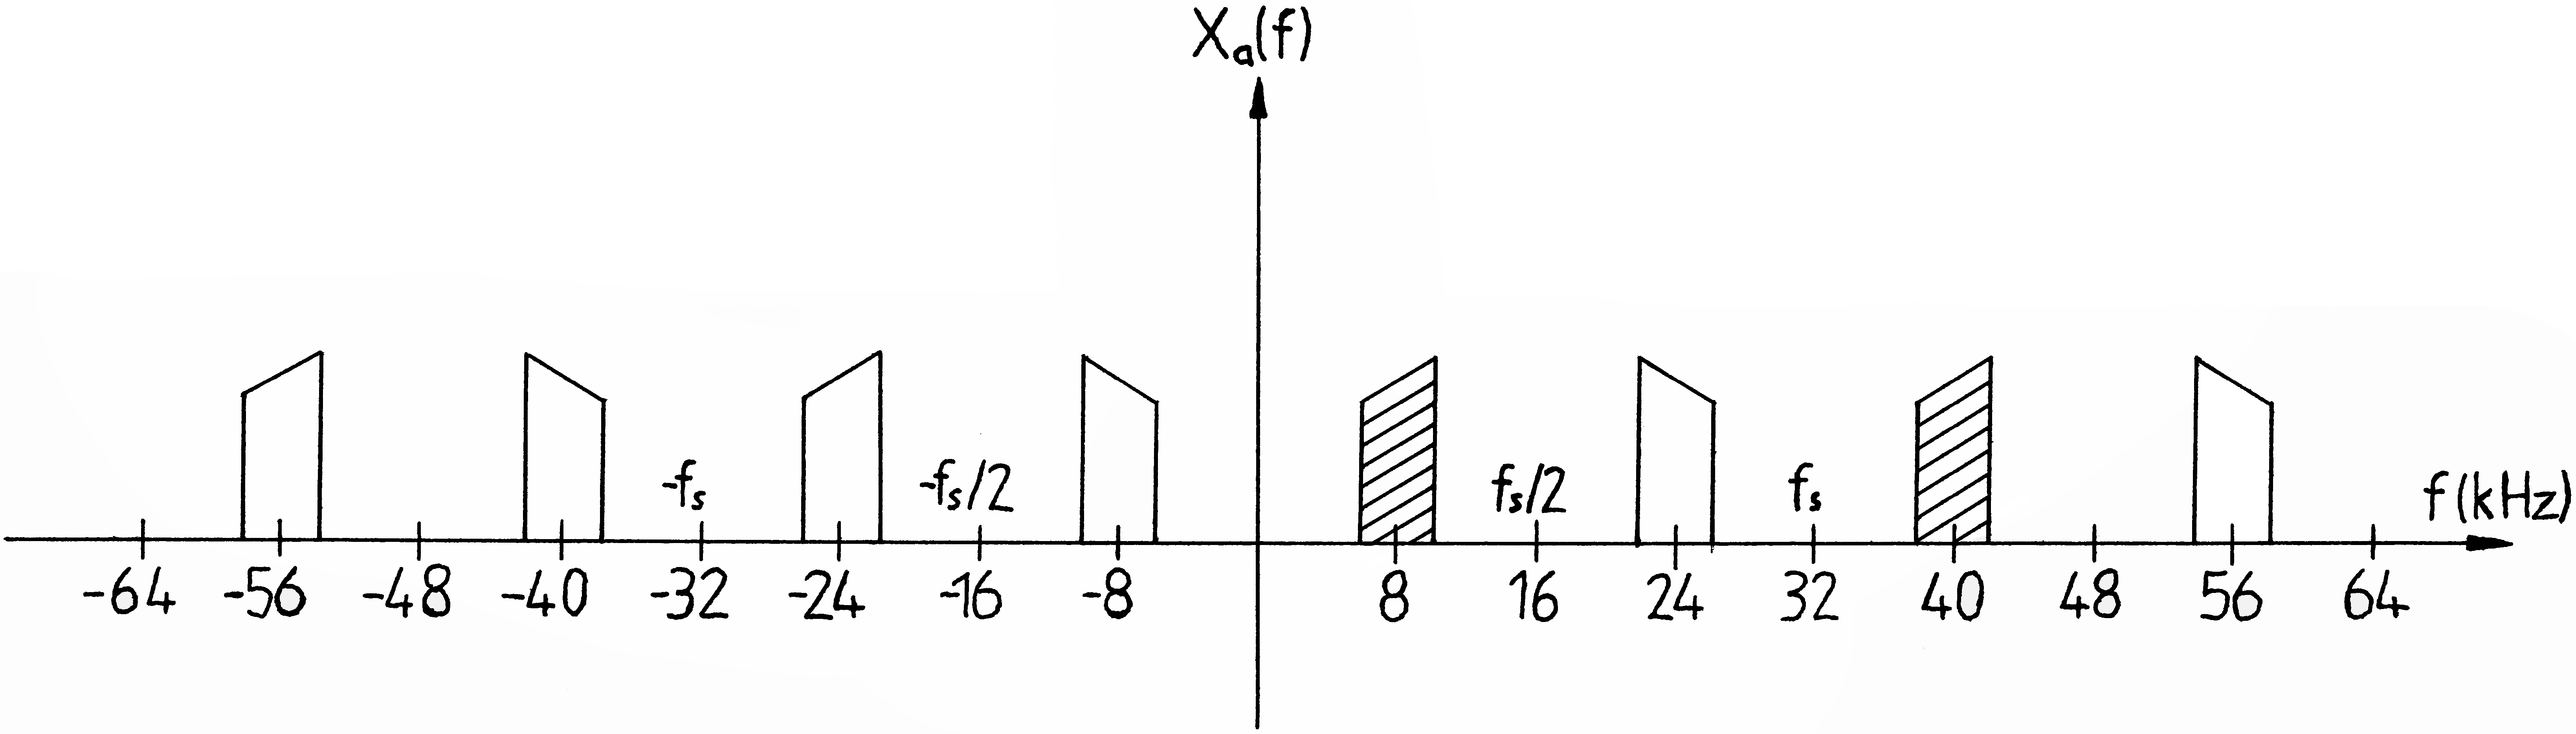
\includegraphics[width=\textwidth]{graphics/image_grundlagen_unterabtastung.png}
\end{center}
\caption{Signal nach der Unterabtastung mit $fs = 32 \mathrm{kHz}$} % picture caption
\label{fig:image_grundlagen_unterabtastung}
\end{figure}
%
%(Abb. \ref{fig:image1})
%%%%%%%%%%%%%%%%%%%%%%%%%%%%%%%%%%%%%%%%%%%%%%%%%%%%%%%%%%%%%%%%%%%%%%%%%%%%%%%%

Erhöht man die Abtastrate nach dem Sampling um den Faktor $R = 4$ auf eine Frequenz von $fs = 128 \mathrm{kHz}$, kann das ursprüngliche Signal bei $40 \mathrm{kHz}$ wiederhergestellt werden. Damit ist die Phaseninformation des Signals wiederherstellbar, sofern bei der Unterabtastung kein Aliasing entsteht.

Das Upsampling im Zeitbereich ist im Prinzip ein Einfügen von Nullen zwischen den vorhandenen Sampling-Werten. Damit wird die Abtastrate für $R$ Nullen zwischen den Werten um den Faktor $R + 1$ erhöht.

Nach dem Upsampling muss mittels geeignetem Filter diejenige Kopie des Signals herausgefiltert werden, die im ursprünglichen Frequenzbereich liegt (das Signal bei $40 \mathrm{kHz}$).
Wegen der schmalbandigen Signale der Ultraschallsensoren kann dafür ein relativ breitbandiges IIR-Bandpassfilter verwendet werden, ohne dass Aliasing entsteht. Beim Filterdesign ist darauf zu achten, dass das Filter nicht schmalbandiger ist als das Signal, sonst würde dieses verfälscht. Jedoch müssen die Kopien bei  $40 \mathrm{kHz} \pm 16 \mathrm{kHz}$ trotzdem genügend gedämpft sein, so dass sie nicht in Erscheinung treten.

Da die Verarbeitung nicht in Echtzeit geschehen muss, kann mithilfe der Funktion \texttt{filtfilt()} das Signal zeitlich in beide Richtungen gefiltert und so ein akausales Filter ohne Phasenverzerrungen erzielt werden.

\subsubsection{Upsampling im Frequenzbereich}\label{sec:upsampling_im_frequenzbereich}
Wie in Abbildung \ref{fig:image_grundlagen_unterabtastung} zu sehen ist, erscheint das Ultraschallsignal vor dem Upsampling als Signal bei $\pm 8 \mathrm{kHz}$. Das ursprüngliche Signal hätte Komponenten bei $\pm 40 \mathrm{kHz}$.
Wird vom unterabgetasteten Signal die FFT berechnet, so kann mit diesen Werten das Spektrum des Signals mit der erhöhten Abtastfrequenz zusammengesetzt werden. Dieser Vorgang ist in Abbildung \ref{fig:image_grundlagen_unterabtastung} zu sehen. Das Spektrum des ursprünglichen Signals (siehe Abbildung \ref{fig:image_grundlagen_upsampling} oben) wird durch Einfügen von Nullen an den richtigen Stellen (rot) zu einem um den Upsampling Faktor $R = 4$ grösseren Frequenzvektor erweitert. Ein Ausschnitt des Frequenzvektors ist in Abbildung \ref{fig:image_grundlagen_upsampling} unten zu sehen. Wird dieses Signal zurück in den Zeitbereich transformiert, so entsteht dadurch das Zeitsignal mit erhöhter Abtastfrequenz.

%%%%%%%%%%%%%%%%%%%%%%%%%%%%%%%%%%%%%%%%%%%%%%%%%%%%%%%%%%%%%%%%%%%%%%%%%%%%%%%%
% pictures
\begin{figure}[htb]
\begin{center}
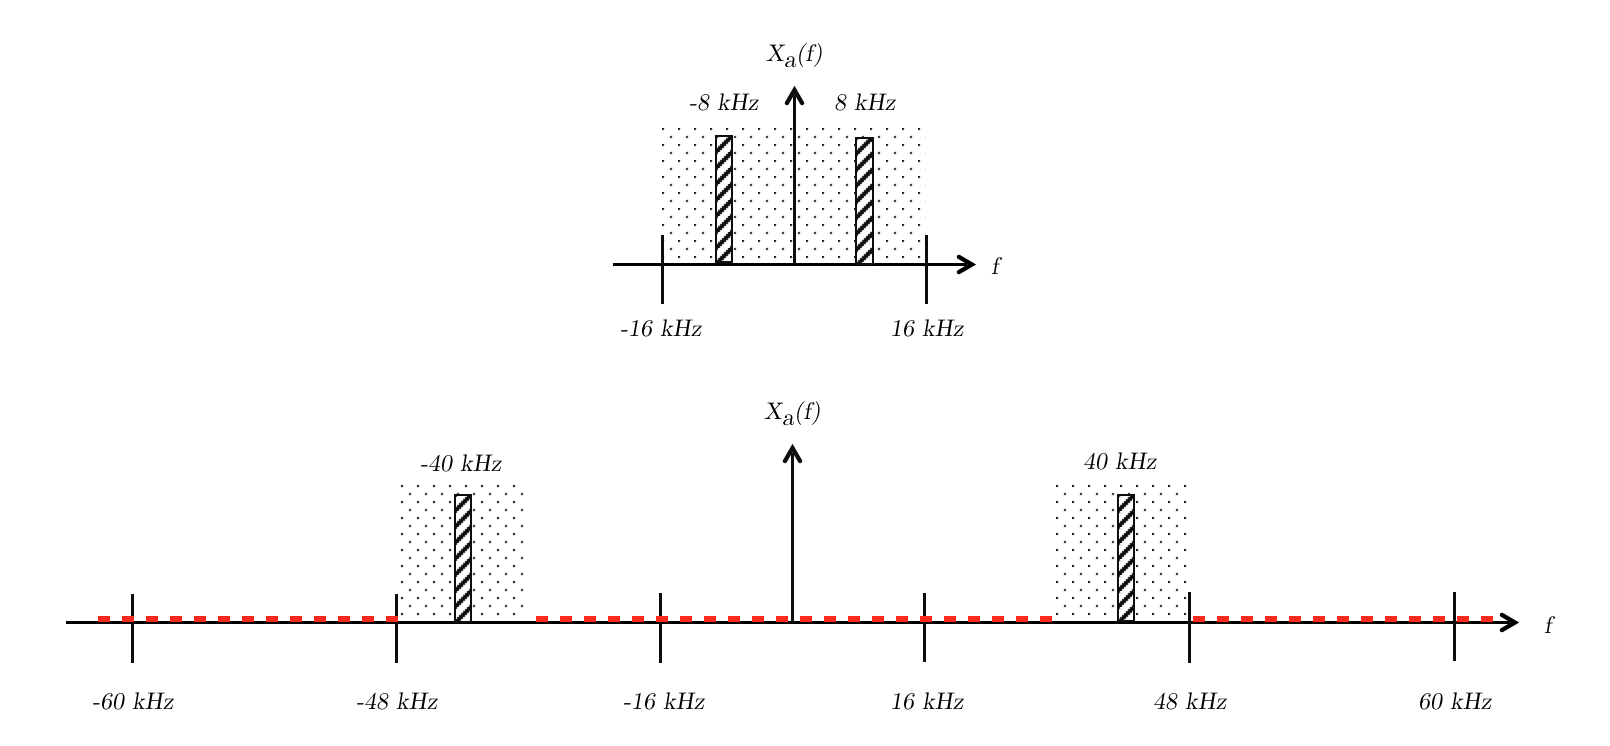
\includegraphics[width=\textwidth]{graphics/image_grundlagen_upsampling.png}
\end{center}
\caption{Upsampling des unterabgetasteten Ultraschallsignals im Frequenzbereich} % picture caption
\label{fig:image_grundlagen_upsampling}
\end{figure}
%
%(Abb. \ref{fig:image1})
%%%%%%%%%%%%%%%%%%%%%%%%%%%%%%%%%%%%%%%%%%%%%%%%%%%%%%%%%%%%%%%%%%%%%%%%%%%%%%%%

Der Vorteil dieser Variante ist, dass auf das Filtern des Signals mit erhöhter Abtastfrequenz im Zeitbereich verzichtet und dadurch Rechenleistung eingespart werden kann.

\subsubsection{Beamforming}\label{sec:beamforming}
Werden die digitalisierten Signale der Ultraschallsensoren addiert, entsteht dadurch eine Richtwirkung des Empfängers mit Haupt- und Nebenkeulen: Durch die Addition der einzelnen Signale der Kanäle addieren sich diejenigen Anteile am stärksten, die in Phase sind. Dies entspricht Schall, der senkrecht auf das Array auftrifft. Um Schall aus einer bestimmten Richtung zu empfangen, werden die einzelnen Kanäle zeitverzögert, bevor sie aufaddiert werden. So werden die Anteile am grössten, die nach dieser Zeitverzögerung in Phase sind. Der dazugehörige Empfangswinkel lässt sich mit Formel (\ref{eq:zeitverschiebung_phasendrehung}) berechnen.

\subsubsection{Enveloppe berechnen}\label{sec:enveloppe_berechnen}
Im negativen Anteil des komplex konjugierten Spektrums eines reellen Zeitsignals steckt keine weitere Information über das Signal, die nicht im positiven Spektrum vorhanden wäre. Theoretisch kann ein reelles Zeitsignal durch einen komplexen Anteil so erweitert werden, dass dessen Spektrum für negative Frequenzen verschwindet. Ein solches Signal bezeichnet man als analytisches Signal.
Um das analytische Signal zu erzeugen, wird das reelle Zeitsignal $x(t)$ um den imaginären Anteil $j \cdot y(t)$ erweitert. Die Transformation, die aus $x(t)$ das Signal $y(t)$ erzeugt, wird als Hilbert-Transformation bezeichnet. Für eine detaillierte Beschreibung der Hilbert-Transformation wird auf \cite{MEYER} verwiesen.

Dieses komplexe Zeitsignal weist für jede Zeit einen Betrag und eine Phase auf. Der Verlauf der Amplitude stellt direkt die Enveloppe des Signals dar. Aus der Ableitung des Verlaufs der Phase kann der Verlauf der Momentanfrequenz berechnet werden. Der Verlauf des Betrags eines analytischen Signals von einem Ultraschallsignal ist in Abbildung \ref{fig:image_grundlagen_upsampling} dargestellt.

%%%%%%%%%%%%%%%%%%%%%%%%%%%%%%%%%%%%%%%%%%%%%%%%%%%%%%%%%%%%%%%%%%%%%%%%%%%%%%%%
% pictures
\begin{figure}[htb]
\begin{center}
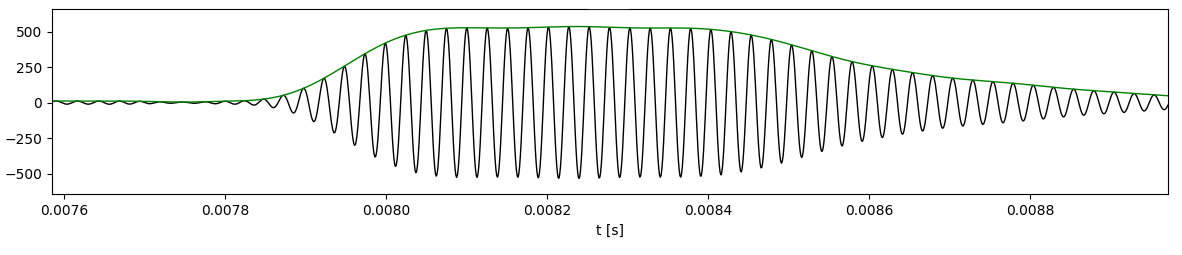
\includegraphics[width=\textwidth]{graphics/image_grundlagen_enveloppe.png}
\end{center}
\caption{Enveloppe eines  Ultraschall-Echos.} % picture caption
\label{fig:image_grundlagen_enveloppe}
\end{figure}
%
%(Abb. \ref{fig:image1})
%%%%%%%%%%%%%%%%%%%%%%%%%%%%%%%%%%%%%%%%%%%%%%%%%%%%%%%%%%%%%%%%%%%%%%%%%%%%%%%%

\subsubsection{Downsampling}\label{sec:downsampling}
Um die Datenmenge zu reduzieren, kann die Abtastfrequenz des Signals um den Faktor $R$ verkleinert werden. Dafür wird nur jeder $R$-te Wert eines Signals berücksichtigt. Die Gesamtdauer des Signals bleibt unverändert.
Die maximal mögliche Frequenz hat sich damit um den Faktor  $R$ verkleinert. Damit kein Aliasing entsteht, müssen im Normalfall störende Frequenzen mit einem Tiefpassfilter unterdrückt werden.

Das zu dezimierende Signal ist die Enveloppe des Ultraschallsignals. Diese ist in Abbildung \ref{fig:image_grundlagen_enveloppe} zu sehen. Weil es sich dabei um ein sehr niederfrequentes Signal handelt, ist kein Tiefpassfilter nötig.
